\documentclass[12pt,a4paper,oneside]{report} %<<<1 ------------------------------
% fonts, encoding:
\usepackage[utf8]{inputenc}             % file is in utf8:
\usepackage{cmap}                       % pdf is created with correct special characters, requires proper font, see next two lines
\usepackage[T1]{fontenc}                % see higher line
\usepackage{tgtermes}                   % high quality times font
\usepackage{textcomp}                   % proper micro sign for SI, use: \textmu, in equation: $\hbox{\textmu}$
\usepackage{slantsc}                   % proper micro sign for SI, use: \textmu, in equation: $\hbox{\textmu}$
\usepackage{calc}                   % provides \widthof
\usepackage{enumitem}                   % provides \begin{description} with settings []
\usepackage{color}                   % provides coloured text
\usepackage{titletoc}                   % multiple contents for examples
% obrazky:
\usepackage{graphicx}                   % to insert pictures
\usepackage{grffile}                    % enables spaces in picture file names
% \grffilesetup{multidot=false, babel=false, encoding, inputencoding=utf8, filenameencoding=utf8, space=true}
\newcommand*{\FILEDOT}{.}                   % if picture file name containt dot (e.g. aaa.bbb.pdf), then TeX considers rest as filename extension, so dot must be written as follows: \includegraphics{aaa\FILEDOT bbb.eps}
% rest:
\usepackage[pdftex,
            unicode,
            pdfauthor={Q-Wave consorcium},
            pdftitle={QWTB documentation: implemented algorithms},
            pdfkeywords={algorithm, data procesing, sampling, toolbox},
            pdfproducer={Latex with hyperref},
            pdfcreator={pdflatex}]{hyperref}
%\usepackage[a4paper]{geometry}          % ensure A4
%\geometry{verbose,lmargin=2.5cm,rmargin=2.5cm,tmargin=2.5cm,bmargin=2.5cm}      % margins settings
\usepackage{url}                        % enables \url in bibtex
%\usepackage{setspace} \doublespacing   % double line spacing, for 1.5 set \onehalfspace
\usepackage{xspace}                     % proper automatic spacing after user defined commands
\usepackage{amsmath}                    % better equations

% chapter/section settings %<<<1 ----------------------------------------------------
\usepackage{titlesec}
%\titleformat*{\section}{\color{blue}{\itshape}}
\titleformat{\chapter}[display]
{\normalfont\bfseries\Huge\filcenter}
{}
{-0.5em}
{}

\titleformat{\section}[display]
{\normalfont\Large\filcenter}
{}
{-0.75em}
{\vspace{1em}\titlerule[1pt]\vspace{0.4em}}

\pagestyle{headings}

% lstlisting settings %<<<1 ----------------------------------------------------
\usepackage{listings}                   % for source code formatting
\definecolor{mygreen}{rgb}{0,0.6,0}
\definecolor{mygray}{rgb}{0.5,0.5,0.5}
\definecolor{lightgray}{rgb}{0.95,0.95,0.95}
\definecolor{mymauve}{rgb}{0.58,0,0.82}

\lstdefinestyle{mcode}{
%\lstset{ %
  backgroundcolor=\color{lightgray},   % choose the background color; you must add \usepackage{color} or \usepackage{xcolor}
  basicstyle=\normalsize\ttfamily,        % the size of the fonts that are used for the code
  breakatwhitespace=false,         % sets if automatic breaks should only happen at whitespace
  breaklines=true,                 % sets automatic line breaking
  captionpos=b,                    % sets the caption-position to bottom
  commentstyle=\color{mygreen},    % comment style
  deletekeywords={...},            % if you want to delete keywords from the given language
  escapeinside={\%*}{*)},          % if you want to add LaTeX within your code
  extendedchars=true,              % lets you use non-ASCII characters; for 8-bits encodings only, does not work with UTF-8
  frame=single,	                   % adds a frame around the code
  keepspaces=true,                 % keeps spaces in text, useful for keeping indentation of code (possibly needs columns=flexible)
  keywordstyle=\color{blue},       % keyword style
  language=Matlab,                 % the language of the code
  otherkeywords={*,qwtb,qwtbvar,alg_info,alg_wrapper,
        normrnd, alg_test,alg_example,...},           % if you want to add more keywords to the set
  numbers=none,                    % where to put the line-numbers; possible values are (none, left, right)
  numbersep=5pt,                   % how far the line-numbers are from the code
  numberstyle=\tiny\color{mygray}, % the style that is used for the line-numbers
  rulecolor=\color{black},         % if not set, the frame-color may be changed on line-breaks within not-black text (e.g. comments (green here))
  showspaces=false,                % show spaces everywhere adding particular underscores; it overrides 'showstringspaces'
  showstringspaces=false,          % underline spaces within strings only
  showtabs=false,                  % show tabs within strings adding particular underscores
  stepnumber=2,                    % the step between two line-numbers. If it's 1, each line will be numbered
  stringstyle=\color{mymauve},     % string literal style
  tabsize=2,                       % sets default tabsize to 2 spaces
  title=\lstname,                  % show the filename of files included with \lstinputlisting; also try caption instead of title
  belowskip=0pt,                   % skip after end of lstlistings
  columns=fullflexible             % do not generate spaces in wordds to simulate fixedwidth font
}

\lstdefinestyle{output}{
%\lstset{ %
  backgroundcolor=\color{lightgray},   % choose the background color; you must add \usepackage{color} or \usepackage{xcolor}
  basicstyle=\normalsize\ttfamily,        % the size of the fonts that are used for the code
  breakatwhitespace=false,         % sets if automatic breaks should only happen at whitespace
  breaklines=true,                 % sets automatic line breaking
  captionpos=b,                    % sets the caption-position to bottom
  commentstyle=\color{mygreen},    % comment style
  deletekeywords={...},            % if you want to delete keywords from the given language
  escapeinside={\%*}{*)},          % if you want to add LaTeX within your code
  extendedchars=true,              % lets you use non-ASCII characters; for 8-bits encodings only, does not work with UTF-8
  frame=none,	                   % adds a frame around the code
  keepspaces=true,                 % keeps spaces in text, useful for keeping indentation of code (possibly needs columns=flexible)
  keywordstyle=\color{blue},       % keyword style
  language=Matlab,                 % the language of the code
  otherkeywords={*,qwtb,qwtbvar,alg_info,alg_wrapper,alg_test,alg_example,...},           % if you want to add more keywords to the set
  numbers=none,                    % where to put the line-numbers; possible values are (none, left, right)
  numbersep=5pt,                   % how far the line-numbers are from the code
  numberstyle=\tiny\color{mygray}, % the style that is used for the line-numbers
  rulecolor=\color{black},         % if not set, the frame-color may be changed on line-breaks within not-black text (e.g. comments (green here))
  showspaces=false,                % show spaces everywhere adding particular underscores; it overrides 'showstringspaces'
  showstringspaces=false,          % underline spaces within strings only
  showtabs=false,                  % show tabs within strings adding particular underscores
  stepnumber=2,                    % the step between two line-numbers. If it's 1, each line will be numbered
  stringstyle=\color{mymauve},     % string literal style
  tabsize=2,                       % sets default tabsize to 2 spaces
  title=\lstname,                  % show the filename of files included with \lstinputlisting; also try caption instead of title
  belowskip=0pt,                  % skip after end of lstlistings
  xleftmargin=20pt,                      % margin on left side
  columns=fullflexible             % do not generate spaces in wordds to simulate fixedwidth font
}

\lstset{style=mcode}
     % user defined code formatting

% bibliography settings %<<<1 ----------------------------------------------------
\usepackage[english]{babel} % main language of the document must be last
\usepackage[
   backend=biber      % if we want unicode 
  ,style=ieee   % or iso-numeric for numeric citation method          
  ,babel=other        % to support multiple languages in bibliography
  %,sortlocale=cs_CZ   % locale of main language, it is for sorting
  ,sortlocale=en_UK   % locale of main language, it is for sorting
  ,bibencoding=UTF8   % this is necessary only if bibliography file is in different encoding than main document
]{biblatex}

% \bibliography{alllib2}
%\defbibenvironment{bibliography}
%    {\list
%        {[\printfield[labelnumberwidth]{labelnumber}]}
%        {\setlength{\labelwidth}{\labelnumberwidth}
%        \setlength{\leftmargin}{4pt}
%        \setlength{\labelsep}{10pt}
%        \addtolength{\leftmargin}{\labelsep}
%        \setlength{\itemsep}{6pt}
%        \setlength{\parsep}{\bibparsep}}
%        \renewcommand*{\makelabel}[1]{\hss##1}}
%    {\endlist}
%    {\item}

\usepackage[yyyymmdd]{datetime}         % command \today with sane format
\renewcommand{\dateseparator}{-}        % strictly ISO date format

% shorts: %<<<1 ----------------------------------------------------

\def\Alg{{\sc Algorithm}\xspace}
\def\Algs{{\sc Algorithms}\xspace}
\def\Tb{{\sc Toolbox}\xspace}
\def\Da{{\sc Data}\xspace}
\def\Mea{{\sc Measurement}\xspace}
\def\Qua{{\sc Quantity}\xspace}
\def\Quas{{\sc Quantities}\xspace}
\def\Wr{{\sc Wrapper}\xspace}
\def\Wrs{{\sc Wrappers}\xspace}
\def\matlab{{\sc MATLAB}\xspace}
\def\octave{{\sc GNU Octave}\xspace}
\def\labview{{\sc LabVIEW}\xspace}
\def\mgo{\matlab/\octave\xspace}
        
\begin{document} % other document settings --------------------------------------------%<<<1
% how to devide special words, e.g. auto-mation
\hyphenation{Frame-work OpenOffice SourceForge Windows}
%\def\thesection{\Roman{section}}       % redefines numbering style of sections
\renewcommand\floatpagefraction{.9} \renewcommand\topfraction{.9} \renewcommand\bottomfraction{.9} \renewcommand\textfraction{.1} \setcounter{totalnumber}{50} \setcounter{topnumber}{50} \setcounter{bottomnumber}{50} % if too many pictures, change text/float fraction
\renewcommand{\labelitemi}{--}          % item sepparator
\setlength{\unitlength}{1mm}            % default length in picture environment

% tight description environment:
\newenvironment{tightdesc}{\begin{description}[itemsep=0pt]} 
                              {\end{description}}

% names of sections:
\def\infosection{Description}
\def\examplesection{Example}
% remove "chapter" from chapter heading:
\renewcommand{\chaptername}{}

\title{QWTB documentation: implemented algorithms}
\author{Q-Wave consorcium}

% first page ----------------------------------------------------------------------- %<<<1 ------------------------------
\thispagestyle{empty}
\begin{center}
        \vspace*{10em}
        {\huge
        \includegraphics[width=0.3\textwidth]{logo/qwtb_logo.png}

        \vspace{2.0em}
        QWTB documentation\\

        \vspace{1.5em}
        Implemented algorithms}\\

        \vfill
        {\Large \color{red}{\today}}

        \vspace{1em}
        {\Large \url{https://qwtb.github.io/qwtb/}}
\end{center}
\newpage

\startcontents[maintoc]
\printcontents[maintoc]{}{0}{\section*{Contents}\setcounter{tocdepth}{2}}

\chapter{Introduction} %<<<1 ------------------------------
This document gives overview of the algorithms implemented in toolbox QWTB.

Toolbox was realized within the EMRP-Project SIB59 Q-Wave. The EMRP is jointly funded by the EMRP
par- ticipating countries within EURAMET and the European Union.

\vspace{4em}
\includegraphics[width=0.3\textwidth]{sources/Q-Wave_logo_01.pdf}
\hfill
\includegraphics[width=0.3\textwidth]{sources/eurametlogo.jpg}

% testing algorithms - normally commented: %<<<1 ------------------------------
% \chapter{testG -- testG} 
% % included files are automatically generated by info_all_algs.m script and by Matlab publish
% % function and converted by bash script betterpublish.
% \section*{\infosection}
% \input{algs_info_published/info_testG.tex}
% \section*{\examplesection}
% \startcontents[localtoc]
\printcontents[localtoc]{}{0}{\subsection*{Contents}\setcounter{tocdepth}{2}}



\phantomsection
\addcontentsline{toc}{section}{Generate sample data}
\subsubsection*{Generate sample data}



Two quantities are prepared: \texttt{x} and \texttt{y}.

\begin{lstlisting}
x = []; y = [];
x.v = [1:20];
y.v = [1:14 13:-1:8];
\end{lstlisting}


All uncertainties are set to 1.

\begin{lstlisting}
x.u = x.v.*0 + 1;
y.u = y.v.*0 + 1;
\end{lstlisting}


Set degrees of freedom.

\begin{lstlisting}
x.d = x.v.*0 + 60;
y.d = y.v.*0 + 9;
\end{lstlisting}


Quantities are put into data input structure \texttt{DI}.

\begin{lstlisting}
DI = [];
DI.x = x;
DI.y = y;
\end{lstlisting}


Create calculation settings \texttt{CS} and set uncertainty calculation method to GUM uncertainty
framework.

\begin{lstlisting}
CS = [];
CS.unc = 'guf';
\end{lstlisting}


\phantomsection
\addcontentsline{toc}{section}{Call algorithm}
\subsubsection*{Call algorithm}



Use QWTB to apply algorithm \texttt{testG} to data \texttt{DI} with calculation settings \texttt{CS}.

\begin{lstlisting}
DO = qwtb('testG', DI, CS);
\end{lstlisting}
\begin{lstlisting}[language={},xleftmargin=5pt,frame=none]
QWTB: default correlation matrix generated for quantity `x`
QWTB: default correlation matrix generated for quantity `y`
QWTB: uncertainty calculation by means of wrapper or algorithm

\end{lstlisting}


\phantomsection
\addcontentsline{toc}{section}{Plot results}
\subsubsection*{Plot results}



Plot input data and calculated maximal and minimal values as a red and green lines with
uncertainties represented by dashed lines.

\begin{lstlisting}
figure
hold on
errorbar(DI.x.v, DI.y.v, DI.y.u, 'xb')
plot([DI.x.v(1) DI.x.v(end)], [DO.max.v DO.max.v], '-r', 'linewidth', 3)
plot([DI.x.v(1) DI.x.v(end)], [DO.max.v - DO.max.u DO.max.v - DO.max.u], '--r', 'linewidth', 3)
plot([DI.x.v(1) DI.x.v(end)], [DO.min.v DO.min.v], '-g', 'linewidth', 3)
plot([DI.x.v(1) DI.x.v(end)], [DO.min.v - DO.min.u DO.min.v - DO.min.u], '--g', 'linewidth', 3)
plot([DI.x.v(1) DI.x.v(end)], [DO.max.v + DO.max.u DO.max.v + DO.max.u], '--r', 'linewidth', 3)
plot([DI.x.v(1) DI.x.v(end)], [DO.min.v + DO.min.u DO.min.v + DO.min.u], '--g', 'linewidth', 3)
legend('original data (DI.x.v, DI.y.v)', 'line at maximum value (DO.max.v)', 'uncertainty',  'line at minimum value (DO.min.v)', 'uncertainty', 'location', 'southoutside')
xlabel('quantity x')
ylabel('quantity y')
title('input data and results of testG algorithm')
hold off
\end{lstlisting}
\begin{center}
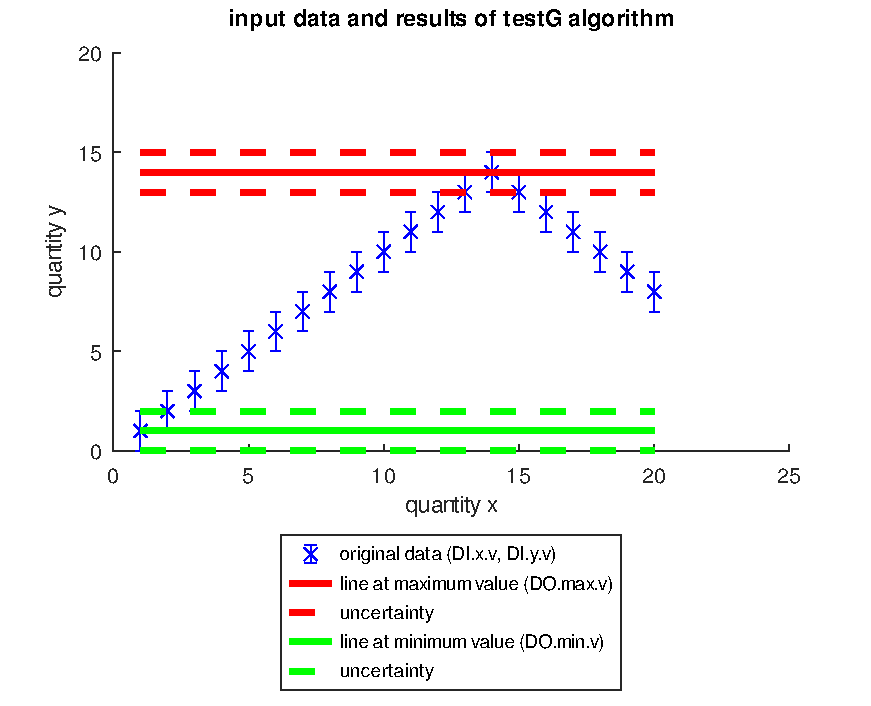
\includegraphics[width=0.7\textwidth]{algs_examples_published/testG_alg_example-1.pdf}
\end{center}


\stopcontents[localtoc]

% 
% \chapter{testGM -- testGM} 
% % included files are automatically generated by info_all_algs.m script and by Matlab publish
% % function and converted by bash script betterpublish.
% \section*{\infosection} 
% \input{algs_info_published/info_testGM.tex}
% \section*{\examplesection}
% \startcontents[localtoc]
\printcontents[localtoc]{}{0}{\subsection*{Contents}\setcounter{tocdepth}{2}}



\phantomsection
\addcontentsline{toc}{section}{Generate sample data}
\subsubsection*{Generate sample data}



Two quantities are prepared: \texttt{x} and \texttt{y}.

\begin{lstlisting}
x = []; y = [];
x.v = [1:20];
y.v = [1:14 13:-1:8];
\end{lstlisting}


All uncertainties are set to 1.

\begin{lstlisting}
x.u = x.v.*0 + 1;
y.u = y.v.*0 + 1;
\end{lstlisting}


Set degrees of freedom.

\begin{lstlisting}
x.d = x.v.*0 + 60;
y.d = y.v.*0 + 9;
\end{lstlisting}


Quantities are put into data input structure \texttt{DI}.

\begin{lstlisting}
DI = [];
DI.x = x;
DI.y = y;
\end{lstlisting}


Create calculation settings \texttt{CS} and set uncertainty calculation method to Monte Carlo method.
Allow randomization of uncertainties by the QWTB toolbox.

\begin{lstlisting}
CSMCM = [];
CSMCM.unc = 'mcm';
CSMCM.mcm.randomize = 1;
\end{lstlisting}


Create calculation settings and set uncertainty calculation method to GUM uncertainty framework.

\begin{lstlisting}
CSGUF = [];
CSGUF.unc = 'guf';
\end{lstlisting}


\phantomsection
\addcontentsline{toc}{section}{Call algorithm}
\subsubsection*{Call algorithm}



Use QWTB to apply algorithm \texttt{testGM} to data \texttt{DI} with calculation settings \texttt{CSGUF}.

\begin{lstlisting}
DOGUF = qwtb('testGM', DI, CSGUF);
\end{lstlisting}
\begin{lstlisting}[language={},xleftmargin=5pt,frame=none]
QWTB: default correlation matrix generated for quantity `x`
QWTB: default correlation matrix generated for quantity `y`
QWTB: uncertainty calculation by means of wrapper or algorithm

\end{lstlisting}


Use QWTB to apply algorithm \texttt{testGM} to data \texttt{DI} with calculation settings \texttt{CSMCM}.

\begin{lstlisting}
DOMCM = qwtb('testGM', DI, CSMCM);
\end{lstlisting}
\begin{lstlisting}[language={},xleftmargin=5pt,frame=none]
QWTB: default correlation matrix generated for quantity `x`
QWTB: default correlation matrix generated for quantity `y`
QWTB: uncertainty calculation by means of wrapper or algorithm

\end{lstlisting}


\phantomsection
\addcontentsline{toc}{section}{Plot results}
\subsubsection*{Plot results}



Plot input data and calculated maximal and minimal values as a red and green lines with
uncertainties represented by dashed lines.

\begin{lstlisting}
figure
hold on
errorbar(DI.x.v, DI.y.v, DI.y.u, 'xb')
plot([DI.x.v(1) DI.x.v(end)], [DOGUF.max.v DOGUF.max.v], '-r', 'linewidth', 3)
plot([DI.x.v(1) DI.x.v(end)], [DOGUF.max.v - DOGUF.max.u DOGUF.max.v - DOGUF.max.u], '--r', 'linewidth', 3)
plot([DI.x.v(1) DI.x.v(end)], [DOGUF.min.v DOGUF.min.v], '-g', 'linewidth', 3)
plot([DI.x.v(1) DI.x.v(end)], [DOGUF.min.v - DOGUF.min.u DOGUF.min.v - DOGUF.min.u], '--g', 'linewidth', 3)
plot([DI.x.v(1) DI.x.v(end)], [DOGUF.max.v + DOGUF.max.u DOGUF.max.v + DOGUF.max.u], '--r', 'linewidth', 3)
plot([DI.x.v(1) DI.x.v(end)], [DOGUF.min.v + DOGUF.min.u DOGUF.min.v + DOGUF.min.u], '--g', 'linewidth', 3)
legend('original data (DI.x.v, DI.y.v)', 'line at maximum value (DO.max.v)', 'uncertainty',  'line at minimum value (DO.min.v)', 'uncertainty', 'location', 'southoutside')
xlabel('quantity x')
ylabel('quantity y')
title('input data and results of testGM algorithm, GUF method')
hold off
\end{lstlisting}
\begin{center}
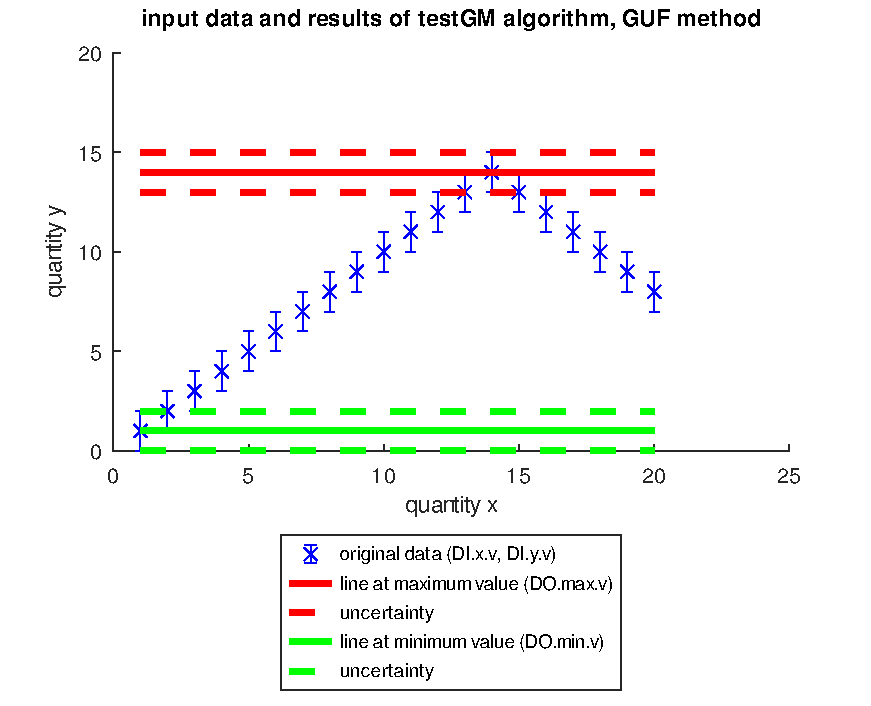
\includegraphics[width=0.7\textwidth]{algs_examples_published/testGM_alg_example-1.pdf}
\end{center}


Plot histogram of calculated maximal value, i.e. probability density function simulated by Monte
Carlo method and overlay by result of GUF method (approximately scaled to MCM result).

\begin{lstlisting}
figure
hold on
hist(DOMCM.max.r, 50)
a = axis;
x = [a(1):0.1:a(2)];
pdf = normpdf(x, DOGUF.max.v, DOGUF.max.u);
plot(x, a(4)/max(pdf).*pdf, '-r', 'linewidth', 4);
title('results of maximum value (DO.max.r)')
legend('Monte Carlo results', 'GUF result (approximately scaled to MCM results', 'location', 'southoutside')
hold off
\end{lstlisting}
\begin{center}
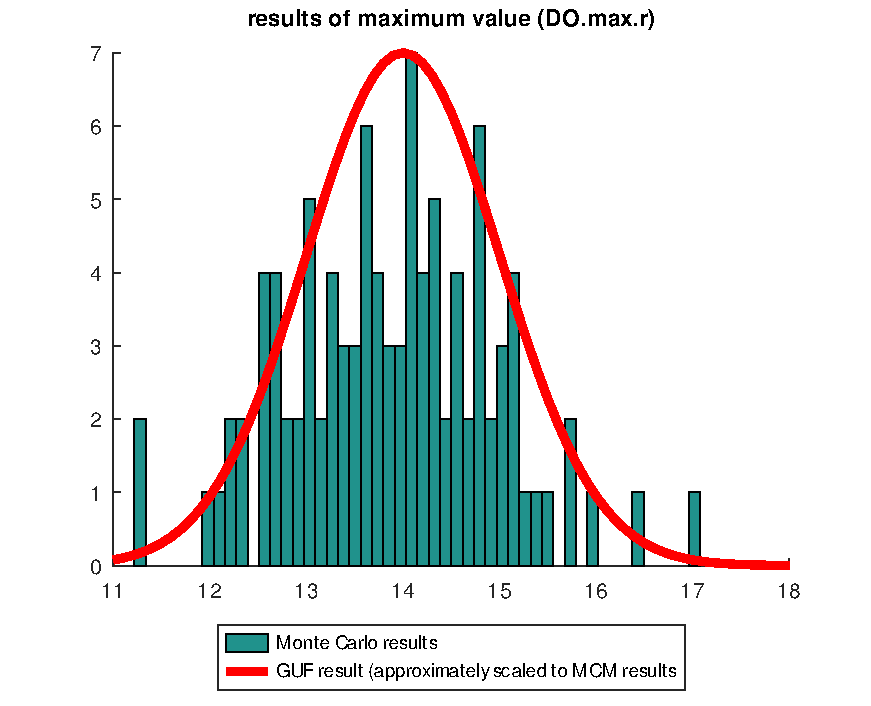
\includegraphics[width=0.7\textwidth]{algs_examples_published/testGM_alg_example-2.pdf}
\end{center}


\stopcontents[localtoc]

% 
% \chapter{testM -- testM} 
% % included files are automatically generated by info_all_algs.m script and by Matlab publish
% % function and converted by bash script betterpublish.
% \section*{\infosection} 
% \input{algs_info_published/info_testM.tex}
% \section*{\examplesection}
% \startcontents[localtoc]
\printcontents[localtoc]{}{0}{\subsection*{Contents}\setcounter{tocdepth}{2}}



\phantomsection
\addcontentsline{toc}{section}{Generate sample data}
\subsubsection*{Generate sample data}



Two quantities are prepared: \texttt{x} and \texttt{y}.

\begin{lstlisting}
x = []; y = [];
x.v = [1:20];
y.v = [1:14 13:-1:8];
\end{lstlisting}


All uncertainties are set to 1.

\begin{lstlisting}
x.u = x.v.*0 + 1;
y.u = y.v.*0 + 1;
\end{lstlisting}


Quantities are put into data input structure \texttt{DI}.

\begin{lstlisting}
DI = [];
DI.x = x;
DI.y = y;
\end{lstlisting}


Create calculation settings \texttt{CS} and set uncertainty calculation method to Monte Carlo method.
Allow randomization of uncertainties by the QWTB toolbox.

\begin{lstlisting}
CS = [];
CS.unc = 'mcm';
CS.mcm.randomize = 1;
\end{lstlisting}


\phantomsection
\addcontentsline{toc}{section}{Call algorithm}
\subsubsection*{Call algorithm}



Use QWTB to apply algorithm \texttt{testM} to data \texttt{DI} with calculation settings \texttt{CS}.

\begin{lstlisting}
DO = qwtb('testM', DI, CS);
\end{lstlisting}
\begin{lstlisting}[language={},xleftmargin=5pt,frame=none]
QWTB: default correlation matrix generated for quantity `x`
QWTB: default correlation matrix generated for quantity `y`
QWTB: uncertainty calculation by means of wrapper or algorithm

\end{lstlisting}


\phantomsection
\addcontentsline{toc}{section}{Plot results}
\subsubsection*{Plot results}



Plot input data and calculated maximal and minimal values as a red and green lines with
uncertainties represented by dashed lines.

\begin{lstlisting}
figure
hold on
errorbar(DI.x.v, DI.y.v, DI.y.u, 'xb')
plot([DI.x.v(1) DI.x.v(end)], [DO.max.v DO.max.v], '-r', 'linewidth', 3)
plot([DI.x.v(1) DI.x.v(end)], [DO.max.v - DO.max.u DO.max.v - DO.max.u], '--r', 'linewidth', 3)
plot([DI.x.v(1) DI.x.v(end)], [DO.min.v DO.min.v], '-g', 'linewidth', 3)
plot([DI.x.v(1) DI.x.v(end)], [DO.min.v - DO.min.u DO.min.v - DO.min.u], '--g', 'linewidth', 3)
plot([DI.x.v(1) DI.x.v(end)], [DO.max.v + DO.max.u DO.max.v + DO.max.u], '--r', 'linewidth', 3)
plot([DI.x.v(1) DI.x.v(end)], [DO.min.v + DO.min.u DO.min.v + DO.min.u], '--g', 'linewidth', 3)
legend('original data (DI.x.v, DI.y.v)', 'line at maximum value (DO.max.v)', 'uncertainty',  'line at minimum value (DO.min.v)', 'uncertainty', 'location', 'southoutside')
xlabel('quantity x')
ylabel('quantity y')
title('input data and results of testM algorithm')
hold off
\end{lstlisting}
\begin{center}
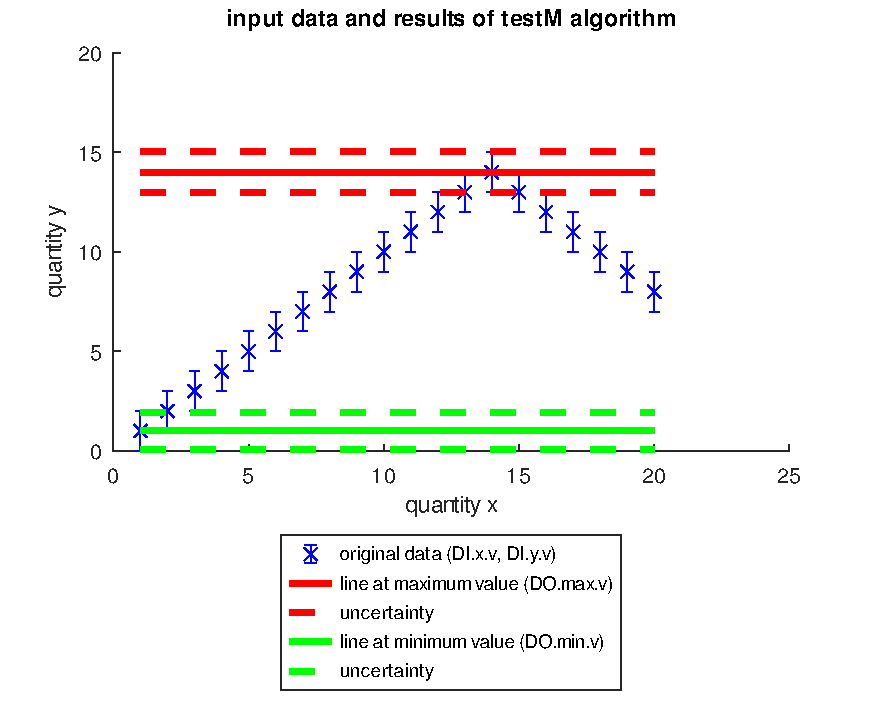
\includegraphics[width=0.7\textwidth]{algs_examples_published/testM_alg_example-1.pdf}
\end{center}


Plot histogram of calculated maximal value, i.e. probability density function simulated by Monte
Carlo method.

\begin{lstlisting}
figure
hist(DO.max.r, 50)
title('histogram of Monte Carlo method results of maximum value (DO.max.r)')
\end{lstlisting}
\begin{center}
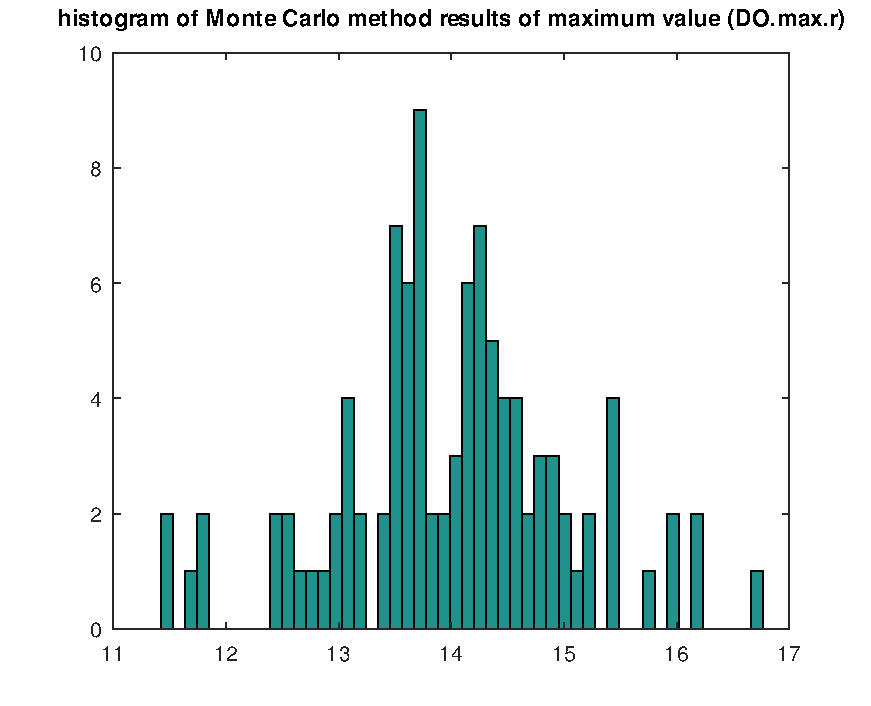
\includegraphics[width=0.7\textwidth]{algs_examples_published/testM_alg_example-2.pdf}
\end{center}


\stopcontents[localtoc]

% 
% \chapter{testQ -- testQ}
% % included files are automatically generated by info_all_algs.m script and by Matlab publish
% % function and converted by bash script betterpublish.
% \section*{\infosection}
% \input{algs_info_published/info_testQ.tex}
% \section*{\examplesection}
% %\startcontents[localtoc]
\printcontents[localtoc]{}{0}{\subsection*{Contents}\setcounter{tocdepth}{2}}



\phantomsection
\addcontentsline{toc}{section}{Generate sample data}
\subsubsection*{Generate sample data}



Quantities are prepared.

\begin{lstlisting}
DI = [];
DI.x.v = [-5:-1:-1];
DI.v.v = [1:10];
DI.a.v = 5;
DI.c.v = 'variable c';
\end{lstlisting}


\phantomsection
\addcontentsline{toc}{section}{Call algorithm}
\subsubsection*{Call algorithm}



Use QWTB to apply algorithm \texttt{testQ} to data \texttt{DI}.

\begin{lstlisting}
DO = qwtb('testQ', DI);
\end{lstlisting}
\begin{lstlisting}[language={},xleftmargin=5pt,frame=none]
QWTB: no uncertainty calculation

\end{lstlisting}


The result is value of \texttt{v}:

\begin{lstlisting}
DO.e.v
\end{lstlisting}
\begin{lstlisting}[language={},xleftmargin=5pt,frame=none]
ans = [](0x0)

\end{lstlisting}


\phantomsection
\addcontentsline{toc}{section}{Different input}
\subsubsection*{Different input}



Add quantity \texttt{u}, which has precedence over \texttt{v}:

\begin{lstlisting}
DI.u.v = [100:110];
DO = qwtb('testQ', DI);
\end{lstlisting}
\begin{lstlisting}[language={},xleftmargin=5pt,frame=none]
QWTB: no uncertainty calculation

\end{lstlisting}


The result is value of \texttt{u}:

\begin{lstlisting}
DO.e.v
\end{lstlisting}
\begin{lstlisting}[language={},xleftmargin=5pt,frame=none]
ans = [](0x0)

\end{lstlisting}


\stopcontents[localtoc]


\chapter{ADEV -- Allan Deviation} %<<<1 ------------------------------
\chaptermark{ADEV}
\stopcontents[maintoc]
% included files are automatically generated by info_all_algs.m script and by Matlab publish
% function and converted by bash script betterpublish.
\section*{\infosection} %<<<2 -------------------
\input{algs_info_published/info_ADEV.tex}
\section*{\examplesection} %<<<2 ------------------------
\startcontents[localtoc]
\printcontents[localtoc]{}{0}{\subsection*{Contents}\setcounter{tocdepth}{2}}



\phantomsection
\addcontentsline{toc}{section}{Generate sample data}
\subsubsection*{Generate sample data}



A random numbers with normal probability distribution function will be generated into input data \texttt{DI.y.v}. Next a drift will be added.

\begin{lstlisting}
DI = [];
DI.y.v = 1.5 + 3.*randn(1, 1e3);
DI.y.v = DI.y.v + [1:1:1e3]./100;
\end{lstlisting}


Lets suppose a sampling frequency is 1 Hz. The algorithm will generate all possible tau values automatically.

\begin{lstlisting}
DI.fs.v = 1;
\end{lstlisting}


\phantomsection
\addcontentsline{toc}{section}{Call algorithm}
\subsubsection*{Call algorithm}



Use QWTB to apply algorithm \texttt{ADEV} to data \texttt{DI}.

\begin{lstlisting}
DO = qwtb('ADEV', DI);
\end{lstlisting}
\begin{lstlisting}[language={},xleftmargin=5pt,frame=none]
QWTB: no uncertainty calculation

\end{lstlisting}


\phantomsection
\addcontentsline{toc}{section}{Display results}
\subsubsection*{Display results}



Log log figure is the best to see allan deviation results:

\begin{lstlisting}
figure; hold on
loglog(DO.tau.v, DO.adev.v, '-b')
loglog(DO.tau.v, DO.adev.v + DO.adev.u, '-k')
loglog(DO.tau.v, DO.adev.v - DO.adev.u, '-k')
xlabel('\tau (sec)');
ylabel('\sigma_y(\tau)');
title(['period = ' num2str(1/DI.fs.v)]);
grid('on'); hold off
\end{lstlisting}
\begin{center}
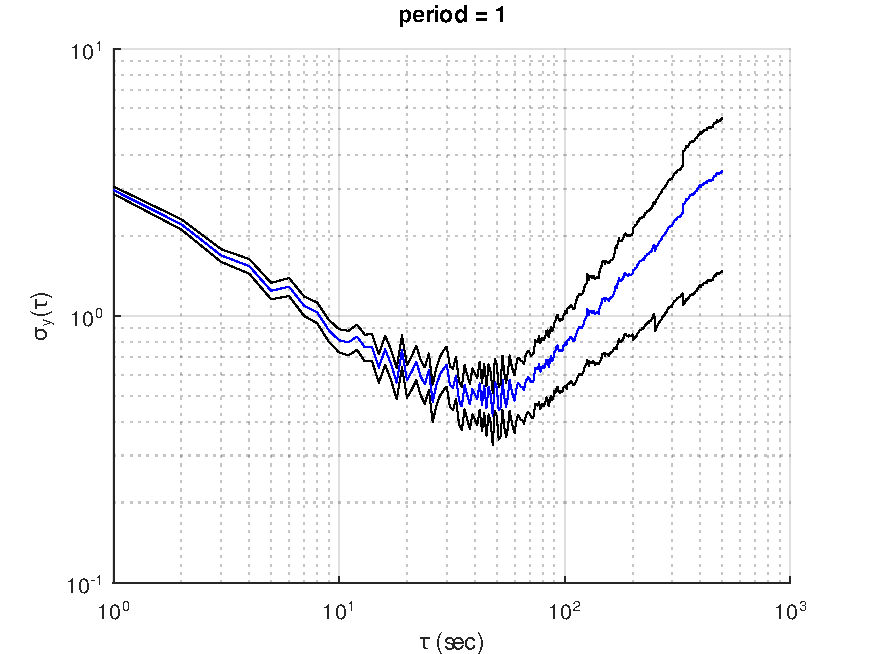
\includegraphics[width=0.7\textwidth]{algs_examples_published/ADEV_alg_example-1.pdf}
\end{center}


\stopcontents[localtoc]

\resumecontents[maintoc]

\chapter{CCC -- Calibration Curves Computing} %<<<1 ------------------------------
\chaptermark{CCC}
\stopcontents[maintoc]
% included files are automatically generated by info_all_algs.m script and by Matlab publish
% function and converted by bash script betterpublish.
\section*{\infosection} %<<<2 -------------------
\begin{tightdesc}
\item [Id:] CCC
\item [Name:] Calibration Curves Computing
\item [Description:] Calibration Curves Computing is a software for the evaluation of instrument calibration curves and developed at Istituto Nazionale di Ricerca Metrologica (INRIM). The software may be applied to pairs of measurement values of independent/explanatory variable and dependent/explained variable. If uncertainties associated with the data are available, they can be provided as inputs to the software. The regression models which can be addressed by the software are (fractional) polynomial curves. The software can perform the following kind of regression procedures: Ordinary least-squares regression (OLS), Weighted least-squares regression (WLS), Weighted total least-squares regression (WTLS).
\item [Citation:] A. Malengo and F. Pennecchi, A weighted total least-squares algorithm for any fitting model with correlated variables, Metrologia (2013), 50, 654.
\item [Remarks:] If |x| and |y| are matrices: wrapper suppose the measured data are a set of groups organized in such that every row of |x| and |y| is one set of measurement, uncertainties in |x| and |y| are neglected and Model 2b is selected. If you want Model 1b or Model 3b, it must be set in quantitiy |model|. If |x| and |y| are vectors: if uncertainties of |x| are zero and uncertainties of |y| contains all the same numbers, Model 1b is selected; if uncertainties of |x| are zero and uncertainties of |y| contains various numbers, Model 2b is selected; if uncertainties of |x| are nonzero Model 3b is selected. In every case the value of |model| overloads automatic determination of the model.
\item [License:] Dedicated license
\item [Provides GUF:] yes
\item [Provides MCM:] no
\item [Input Quantities] \rule{0em}{0em}
    \begin{tightdesc}
    \item [Required:] 
        \textsf{x},\enspace \textsf{y},\enspace \textsf{exponents}
    \item [Optional:] 
        \textsf{model}
    \item [Parameters:] 
        \textsf{exponents},\enspace \textsf{model}
    \item [Descriptions:] \rule{0em}{0em}
        \begin{tightdesc}
            \item[\textsf{exponents}] -- Exponents of polynomial used to fit, from -5 to 5 including 0, -0.5, 0.5
            \item[\textsf{model}] -- Identification of the model. 1a, 2a, 3a, 1b, 2b, 3b.
            \item[\textsf{x}] -- Independent/explanatory variable
            \item[\textsf{y}] -- Dependent/explained variable
        \end{tightdesc}
    \end{tightdesc}
\item [Output Quantities:] \rule{0em}{0em}
    \begin{tightdesc}
        \item[\textsf{coefs}] -- Fitted coefficients
        \item[\textsf{exponents}] -- Exponents of polynomial used to fit, from -5 to 5 including 0, -0.5, 0.5
        \item[\textsf{func}] -- Inline function constructed for exponents with parameters `x` and `coefs.v`
        \item[\textsf{model}] -- Model used for calculation.
        \item[\textsf{yhat}] -- Fitted values y
    \end{tightdesc}
\end{tightdesc}

\section*{\examplesection} %<<<2 ------------------------
\startcontents[localtoc]
\printcontents[localtoc]{}{0}{\subsection*{Contents}\setcounter{tocdepth}{2}}



\phantomsection
\addcontentsline{toc}{section}{Generate sample data}
\subsubsection*{Generate sample data}



An dependence of amplitude error (Volts, ppm) on signal frequency (Hz) of an ADC was measured and
uncertainties of measurement was estimated. The uncertainty of frequency can be considered as
negligible.

\begin{lstlisting}
%3.7+12.*x+3.*x.^2
f = [10 1e2 1e3 1e4 1e5];
err = [19.700 32.700 69.700 90.700 148.700];
err_unc = [4 10 13 20 33];
\end{lstlisting}


Set independent and dependent variables for \texttt{CCC} algorithm. Lets operate in semi logarithm space
for easy plotting.

\begin{lstlisting}
DI = [];
DI.x.v = log10(f);
DI.x.u = [];
DI.y.v = err;
DI.y.u = err_unc;
\end{lstlisting}


Suppose the ADC has quadratic dependence of the error on the signal frequency.

\begin{lstlisting}
DI.exponents.v = [0 1 2];
\end{lstlisting}


\phantomsection
\addcontentsline{toc}{section}{Call algorithm}
\subsubsection*{Call algorithm}



Use QWTB to apply algorithm \texttt{CCC} to data \texttt{DI}.

\begin{lstlisting}
DO = qwtb('CCC', DI);
\end{lstlisting}
\begin{lstlisting}[language={},xleftmargin=5pt,frame=none]
QWTB: no uncertainty calculation
QWTB: CCC wrapper: model was set by CCC wrapper to a value `Model 2a`.
warning: inline is obsolete; use anonymous functions instead

\end{lstlisting}


\phantomsection
\addcontentsline{toc}{section}{Display results}
\subsubsection*{Display results}



Results is

\begin{lstlisting}
disp(['offset          : ' num2str(DO.coefs.v(1)) ' +- ' num2str(DO.coefs.u(1))])
disp(['linear coeff.   : ' num2str(DO.coefs.v(2)) ' +- ' num2str(DO.coefs.u(2))])
disp(['quadratic coeff.: ' num2str(DO.coefs.v(3)) ' +- ' num2str(DO.coefs.u(3))])
\end{lstlisting}
\begin{lstlisting}[language={},xleftmargin=5pt,frame=none]
offset          : 12.6828 +- 16.9884
linear coeff.   : 1.9434 +- 19.1198
quadratic coeff.: 4.9055 +- 3.9754

\end{lstlisting}


\phantomsection
\addcontentsline{toc}{section}{Interpolate values}
\subsubsection*{Interpolate values}



Interpolate fitted polynom at values \texttt{t}.

\begin{lstlisting}
t = [0:0.1:6];
ty = DO.func.v(t, DO.coefs.v);
\end{lstlisting}


Calculate uncertainties of interpolated values (\texttt{S} is sensitivity matrix, \texttt{CC} is covariance
matrix of coefficients, \texttt{CT} is covariance matrix of interpolated values, \texttt{uty} is uncertainty of
interpolated values).

\begin{lstlisting}
for i = 1:length(t);
        S = t(i).^DI.exponents.v;
        CC = diag(DO.coefs.u,0)*DO.coefs.c*diag(DO.coefs.u,0);
        CT(i)=S*CC*S';
end
uty=CT.^0.5;
\end{lstlisting}


\phantomsection
\addcontentsline{toc}{section}{Plot results}
\subsubsection*{Plot results}

\begin{lstlisting}
hold on
errorbar(DI.x.v, DI.y.v, DI.y.u, 'xb')
errorbar(DI.x.v, DO.yhat.v, DO.yhat.u, 'og')
plot(t, ty, '-r');
plot(t, ty + uty, '-r');
plot(t, ty - uty, '-r');
xlabel('log(f)')
ylabel('error of amplitude')
legend('original data','fitted values','interpolated values', 'uncer. of int. val.','location','southeast')
hold off
\end{lstlisting}
\begin{center}
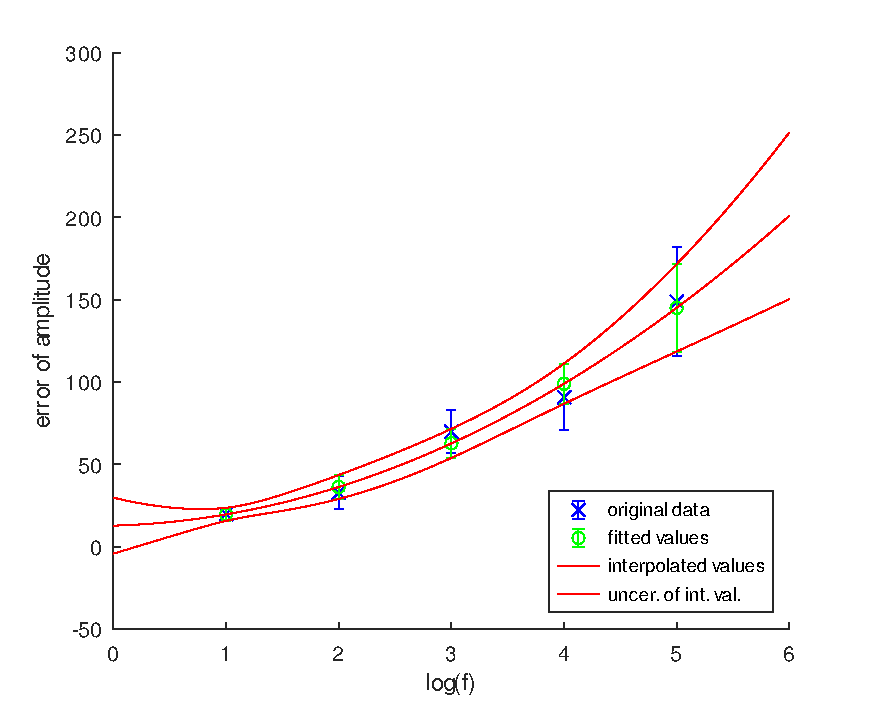
\includegraphics[width=0.7\textwidth]{algs_examples_published/CCC_alg_example-1.pdf}
\end{center}


\stopcontents[localtoc]

\resumecontents[maintoc]

\chapter{FOAV -- Fast Fully Overlapped Allan Variance} %<<<1 ------------------------------
\chaptermark{FFOAV}
\stopcontents[maintoc]
% included files are automatically generated by info_all_algs.m script and by Matlab publish
% function and converted by bash script betterpublish.
\section*{\infosection} %<<<2 -------------------
\begin{tightdesc}
\item [Id:] FFOAV
\item [Name:] Fast Fully Overlapped Allan Variance
\item [Description:] Fast, parallelizeable algorithm to calculate Fully Overlapped Allan Variance for generating smooth Allan Deviation plots whose serial running time is $\Theta(N^2)$.
\item [Citation:] S. M. Yadav, S. K. Shastri, G. B. Chakravarthi, V. Kumar, D. R. A and V. Agrawal, "A Fast, Parallel Algorithm for Fully Overlapped Allan Variance and Total Variance for Analysis and Modelling of Noise in Inertial Sensors," in IEEE Sensors Letters. doi: 10.1109/LSENS.2018.2829799. Github repository: \url{https://github.com/shrikanth95/Fast-Parallel-Fully-Overlapped-Allan-Variance-and-Total-Variance}
\item [Remarks:] If sampling frequency |fs| is not supplied, wrapper will calculate |fs| from sampling time |Ts| or if not supplied, mean of differences of time series |t| is used to calculate |Ts|. The output is recaldulated to return deviation to correspond other algorithms.
\item [License:] MIT License
\item [Provides GUF:] no
\item [Provides MCM:] no
\item [Input Quantities] \rule{0em}{0em}
    \begin{tightdesc}
    \item [Required:] 
        \textsf{fs} or \textsf{Ts} or \textsf{t},\enspace \textsf{y}
    \item [Descriptions:] \rule{0em}{0em}
        \begin{tightdesc}
            \item[\textsf{Ts}] -- Sampling time
            \item[\textsf{fs}] -- Sampling frequency
            \item[\textsf{t}] -- Time series
            \item[\textsf{y}] -- Sampled values
        \end{tightdesc}
    \end{tightdesc}
\item [Output Quantities:] \rule{0em}{0em}
    \begin{tightdesc}
        \item[\textsf{oadev}] -- Overlapped Allan deviation
        \item[\textsf{tau}] -- Observation time of resulted values
    \end{tightdesc}
\end{tightdesc}

\section*{\examplesection} %<<<2 ------------------------
\startcontents[localtoc]
\printcontents[localtoc]{}{0}{\subsection*{Contents}\setcounter{tocdepth}{2}}



\phantomsection
\addcontentsline{toc}{section}{NOT FINISHED! XXX}
\subsubsection*{NOT FINISHED! XXX}



\phantomsection
\addcontentsline{toc}{section}{Generate sample data}
\subsubsection*{Generate sample data}



A random numbers with normal probability distribution function will be generated into input data \texttt{DI.y.v}. Next a drift will be added.

\begin{lstlisting}
DI = [];
DI.y.v = 1.5 + 3.*randn(1, 1e3);
DI.y.v = DI.y.v + [1:1:1e3]./100;
\end{lstlisting}


Lets suppose a sampling frequency is 1 Hz. The algorithm will generate all possible tau values automatically.

\begin{lstlisting}
DI.fs.v = 1;
\end{lstlisting}


\phantomsection
\addcontentsline{toc}{section}{Call algorithm}
\subsubsection*{Call algorithm}



Use QWTB to apply algorithm \texttt{ADEV} to data \texttt{DI}.

\begin{lstlisting}
DO = qwtb('ADEV', DI);
\end{lstlisting}
\begin{lstlisting}[language={},xleftmargin=5pt,frame=none]
QWTB: no uncertainty calculation

\end{lstlisting}


\phantomsection
\addcontentsline{toc}{section}{Display results}
\subsubsection*{Display results}



Log log figure is the best to see allan deviation results:

\begin{lstlisting}
figure; hold on
loglog(DO.tau.v, DO.adev.v, '-b')
loglog(DO.tau.v, DO.adev.v + DO.adev.u, '-k')
loglog(DO.tau.v, DO.adev.v - DO.adev.u, '-k')
xlabel('\tau (sec)');
ylabel('\sigma_y(\tau)');
title(['period = ' num2str(1/DI.fs.v)]);
grid('on'); hold off
\end{lstlisting}
\begin{center}
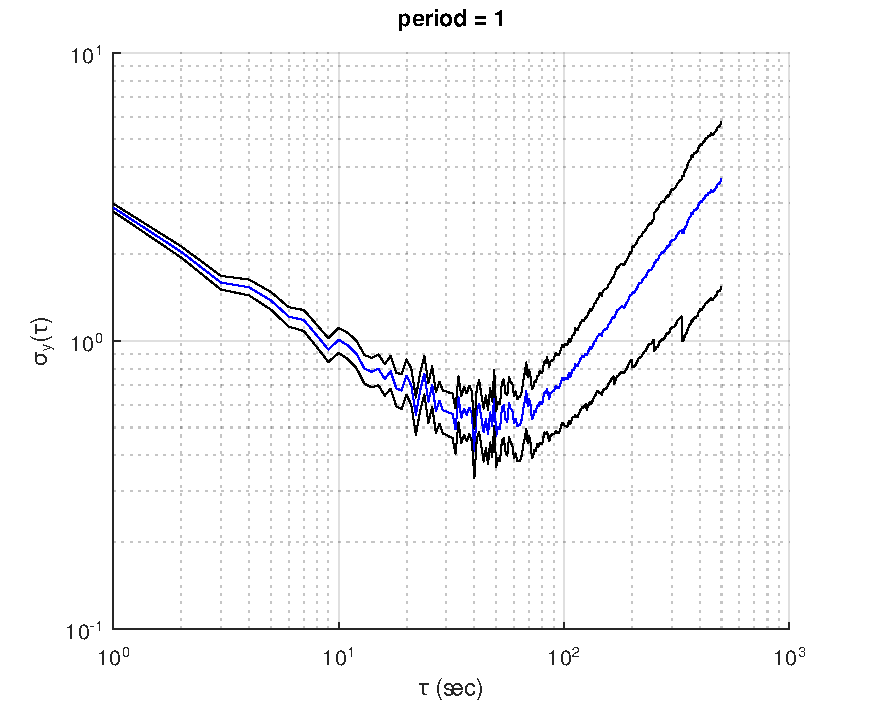
\includegraphics[width=0.7\textwidth]{algs_examples_published/FFOAV_alg_example-1.pdf}
\end{center}


\stopcontents[localtoc]

\resumecontents[maintoc]

\chapter{flicker\_sim -- Flickermeter simulator} %<<<1 ------------------------------
\chaptermark{flicker\_sim}
\stopcontents[maintoc]
% included files are automatically generated by info_all_algs.m script and by Matlab publish
% function and converted by bash script betterpublish.
\section*{\infosection} %<<<2 -------------------
\begin{tightdesc}
\item [Id:] flicker\_sim
\item [Name:] Flickermeter simulator
\item [Description:] Calculates instantaneous flicker sensation Pinst and short-term flicker severity Pst.
\item [Citation:] Implemented according: IEC 61000-4-15, Electromagnetic compatibility (EMC), Testing and measurement techniques, Flickermeter, Edition 2.0, 2010-08; Wilhelm Mombauer: "Messung von Spannungsschwankungen und Flickern mit dem IEC-Flickermeter", ISBN 3-8007-2525-8, VDE-Verlag; Solcept Open Source Flicker Measurement-Simulator \url{https://www.solcept.ch/en/tools/flickersim/;} NPL Reference Flickermeter Design \url{http://www.npl.co.uk/electromagnetics/electrical-measurement/products-and-services/npl-reference-flickermeter-design}
\item [Remarks:] If sampling frequency |fs| is not supplied, wrapper will calculate |fs| from sampling time |Ts| or if not supplied, mean of differences of time series |t| is used to calculate |Ts|. Sampling frequency has to be higher than 7 kHz. If sampling f. is higher than 23 kHz, signal will be down sampled by algorithm. More than 600 s of signal is required. Requires either Signal Processing Toolbox when run in MATLAB or signal package when run in GNU Octave. Frequency of line (carrier frequency) |f\_line| can be only 50 or 60 Hz
\item [License:] Boost Software License
\item [Provides GUF:] no
\item [Provides MCM:] no
\item [Input Quantities] \rule{0em}{0em}
    \begin{tightdesc}
    \item [Required:] 
        \textsf{fs} or \textsf{Ts} or \textsf{t},\enspace \textsf{y},\enspace \textsf{f\_line}
    \item [Descriptions:] \rule{0em}{0em}
        \begin{tightdesc}
            \item[\textsf{Ts}] -- Sampling time
            \item[\textsf{f\_line}] -- Line frequency
            \item[\textsf{fs}] -- Sampling frequency
            \item[\textsf{t}] -- Time series
            \item[\textsf{y}] -- Sampled values
        \end{tightdesc}
    \end{tightdesc}
\item [Output Quantities:] \rule{0em}{0em}
    \begin{tightdesc}
        \item[\textsf{Pinst}] -- Instantaneous flicker sensation
        \item[\textsf{Pst}] -- Short-term flicker severity
    \end{tightdesc}
\end{tightdesc}

\section*{\examplesection} %<<<2 ------------------------
\startcontents[localtoc]
\printcontents[localtoc]{}{0}{\subsection*{Contents}\setcounter{tocdepth}{2}}



\phantomsection
\addcontentsline{toc}{section}{Generate sample data}
\subsubsection*{Generate sample data}



A time series representing voltage measured on a power supply line will be generated. Modulation
amplitude \texttt{dVV} in percents, modulation frequency \texttt{CPM} in changes per minute, line frequency
\texttt{f\_c}, and line amplitude \texttt{A\_c} in volts are selected according Table 5 of EN61000-4-15/A1, line
4, collumn 3. Measurement time \texttt{siglen} and sampling frequency \texttt{f\_s} are selected according
recommendations of algorithm flicker\_sim. Resulted Pst should be very near 1.

\begin{lstlisting}
dVV = 0.894; CPM = 39; A_c = 230.*sqrt(2); f_c = 50; siglen = 720; f_s = 20000;
% Frequency of the modulation (flicker) signal in hertz:
f_F = CPM / ( 60 * 2 );
% Time series:
t = linspace(0, siglen, siglen.*f_s);
% Sampled signal. Modulation is set in such way 10 minutes before end of signal modulation is zero.
y = A_c*sin(2*pi*f_c*t) .* ( 1 + (dVV/100)/2*sign(sin(2*pi*f_F*t - (siglen - 10).*f_F.*2.*pi)) );
\end{lstlisting}


\phantomsection
\addcontentsline{toc}{section}{Set input data.}
\subsubsection*{Set input data.}

\begin{lstlisting}
DI = [];
DI.y.v = y;
DI.fs.v = f_s;
DI.f_line.v = f_c;
\end{lstlisting}


\phantomsection
\addcontentsline{toc}{section}{Call algorithm}
\subsubsection*{Call algorithm}



Use QWTB to apply algorithm \texttt{flicker\_sim} to data \texttt{DI}.

\begin{lstlisting}
DO = qwtb('flicker_sim', DI);
\end{lstlisting}
\begin{lstlisting}[language={},xleftmargin=5pt,frame=none]
QWTB: no uncertainty calculation
warning: Invalid UTF-8 byte sequences have been replaced.
warning: called from
    alg_wrapper at line 25 column 14
    qwtb>check_and_run_alg at line 377 column 17
    qwtb at line 114 column 47
    publish>eval_code_helper at line 1079 column 8
    publish>eval_code at line 995 column 30
    publish at line 402 column 9
    all_algs_examples2tex at line 51 column 5
 

\end{lstlisting}


\phantomsection
\addcontentsline{toc}{section}{Display results}
\subsubsection*{Display results}



Short-term flicker severity:

\begin{lstlisting}
Pst = DO.Pst
% Maximum of instantaneous flicker sensation:
Pinstmax = max(DO.Pinst)
\end{lstlisting}
\begin{lstlisting}[language={},xleftmargin=5pt,frame=none]
error: max: wrong type argument 'scalar struct'
	in:

Pst = DO.Pst
% Maximum of instantaneous flicker sensation:
Pinstmax = max(DO.Pinst)
\end{lstlisting}


\stopcontents[localtoc]

\resumecontents[maintoc]

\chapter{FourPSF -- Standard Four Parameter Sine Wave Fit according IEEE Std 1241-2000} %<<<1 ------------------------------
\chaptermark{FourPSF}
\stopcontents[maintoc]
% included files are automatically generated by info_all_algs.m script and by Matlab publish
% function and converted by bash script betterpublish.
\section*{\infosection} %<<<2 -------------------
\input{algs_info_published/info_FourPSF.tex}
\section*{\examplesection} %<<<2 ------------------------
\startcontents[localtoc]
\printcontents[localtoc]{}{0}{\subsection*{Contents}\setcounter{tocdepth}{2}}



\phantomsection
\addcontentsline{toc}{section}{Generate sample data}
\subsubsection*{Generate sample data}



Two quantities are prepared: \texttt{t} and \texttt{y}, representing 1 second of sinus waveform of nominal
frequency 1 kHz, nominal amplitude 1 V, nominal phase 1 rad and offset 1 V sampled at sampling
frequency 10 kHz.

\begin{lstlisting}
DI = [];
Anom = 2; fnom = 100; phnom = 1; Onom = 0.2;
DI.t.v = [0:1/1e4:1-1/1e4];
DI.y.v = Anom*sin(2*pi*fnom*DI.t.v + phnom) + Onom;
\end{lstlisting}


\phantomsection
\addcontentsline{toc}{section}{Call algorithm}
\subsubsection*{Call algorithm}



Use QWTB to apply algorithm \texttt{FourPSF} to data \texttt{DI}.

\begin{lstlisting}
CS.verbose = 1;
DO = qwtb('FourPSF', DI, CS);
\end{lstlisting}
\begin{lstlisting}[language={},xleftmargin=5pt,frame=none]
QWTB: no uncertainty calculation
QWTB: FourPSF wrapper: sampling time was calculated from time series

\end{lstlisting}


\phantomsection
\addcontentsline{toc}{section}{Display results}
\subsubsection*{Display results}



Results is the amplitude, frequency, phase and offset of sampled waveform.

\begin{lstlisting}
A = DO.A.v
f = DO.f.v
ph = DO.ph.v
O = DO.O.v
\end{lstlisting}
\begin{lstlisting}[language={},xleftmargin=5pt,frame=none]
A = 2.0000
f = 100
ph = 1.0000
O = 0.2000

\end{lstlisting}


Errors of estimation in parts per milion:

\begin{lstlisting}
Aerrppm = (DO.A.v - Anom)/Anom .* 1e6
ferrppm = (DO.f.v - fnom)/fnom .* 1e6
pherrppm = (DO.ph.v - phnom)/phnom .* 1e6
Oerrppm = (DO.O.v - Onom)/Onom .* 1e6
\end{lstlisting}
\begin{lstlisting}[language={},xleftmargin=5pt,frame=none]
Aerrppm = -4.4409e-10
ferrppm = 0
pherrppm = 8.8818e-10
Oerrppm = 5.5511e-10

\end{lstlisting}


\stopcontents[localtoc]

\resumecontents[maintoc]

\chapter{FPNLSF -- Four Parameter Non-Linear Sine Fit} %<<<1 ------------------------------
\chaptermark{FPNLSF}
\stopcontents[maintoc]
% included files are automatically generated by info_all_algs.m script and by Matlab publish
% function and converted by bash script betterpublish.
\section*{\infosection} %<<<2 -------------------
\input{algs_info_published/info_FPNLSF.tex}
\section*{\examplesection} %<<<2 ------------------------
\startcontents[localtoc]
\printcontents[localtoc]{}{0}{\subsection*{Contents}\setcounter{tocdepth}{2}}



\phantomsection
\addcontentsline{toc}{section}{Generate sample data}
\subsubsection*{Generate sample data}



Two quantities are prepared: \texttt{t} and \texttt{y}, representing 1 second of sinus waveform of nominal
frequency 1 kHz, nominal amplitude 1 V, nominal phase 1 rad and offset 1 V sampled at sampling
frequency 10 kHz.

\begin{lstlisting}
DI = [];
Anom = 2; fnom = 100; phnom = 1; Onom = 0.2;
DI.t.v = [0:1/1e4:1-1/1e4];
DI.y.v = Anom*sin(2*pi*fnom*DI.t.v + phnom) + Onom;
\end{lstlisting}


Lets make an estimate of frequency 0.2 percent higher than nominal value:

\begin{lstlisting}
DI.fest.v = 100.2;
\end{lstlisting}


\phantomsection
\addcontentsline{toc}{section}{Call algorithm}
\subsubsection*{Call algorithm}



Use QWTB to apply algorithm \texttt{FPNLSF} to data \texttt{DI}.

\begin{lstlisting}
CS.verbose = 1;
DO = qwtb('FPNLSF', DI, CS);
\end{lstlisting}
\begin{lstlisting}[language={},xleftmargin=5pt,frame=none]
QWTB: no uncertainty calculation
Fitting started
Fitting finished

\end{lstlisting}


\phantomsection
\addcontentsline{toc}{section}{Display results}
\subsubsection*{Display results}



Results is the amplitude, frequency and phase of sampled waveform.

\begin{lstlisting}
A = DO.A.v
f = DO.f.v
ph = DO.ph.v
O = DO.O.v
\end{lstlisting}
\begin{lstlisting}[language={},xleftmargin=5pt,frame=none]
A = 2.0000
f = 100.000
ph = 1.0000
O = 0.2000

\end{lstlisting}


Errors of estimation in parts per milion:

\begin{lstlisting}
Aerrppm = (DO.A.v - Anom)/Anom .* 1e6
ferrppm = (DO.f.v - fnom)/fnom .* 1e6
pherrppm = (DO.ph.v - phnom)/phnom .* 1e6
Oerrppm = (DO.O.v - Onom)/Onom .* 1e6
\end{lstlisting}
\begin{lstlisting}[language={},xleftmargin=5pt,frame=none]
Aerrppm = -7.7716e-10
ferrppm = -4.0927e-08
pherrppm = 5.6228e-06
Oerrppm = -4.1217e-08

\end{lstlisting}


\stopcontents[localtoc]

\resumecontents[maintoc]

\chapter{GenNHarm -- Basic signal generator} %<<<1 ------------------------------
\chaptermark{GenNHarm}
\stopcontents[maintoc]
% included files are automatically generated by info_all_algs.m script and by Matlab publish
% function and converted by bash script betterpublish.
\section*{\infosection} %<<<2 -------------------
\begin{tightdesc}
\item [Id:] GenNHarm
\item [Name:] Basic signal generator
\item [Description:] An algorithm for generating sampled waveforms with multiple harmonic or interharmonic components and noise level.
\item [Citation:] N/A
\item [Remarks:] If times of samples |t| are not defined, wrapper will calculate |t| from: sampling frequency |fs| or sampling period |Ts|, and from: number of samples |L| or number of main signal periods |M|. Vectors |f|, |A|, |ph|, |O| defines harmonic frequencies. First value is the main signal component. If |f|, |A|, |ph|, |O| are scalar, and |thd\_k1|>0 and |nharm|>1, than harmonics are added to the signal to make required |thd\_k1|.
\item [License:] MIT License
\item [Provides GUF:] no
\item [Provides MCM:] no
\item [Input Quantities] \rule{0em}{0em}
    \begin{tightdesc}
    \item [Required:] 
        \textsf{Ts} or \textsf{fs} or \textsf{t}
    \item [Optional:] 
        \textsf{M},\enspace \textsf{noise}
    \item [Parameters:] 
        \textsf{noise}
    \item [Descriptions:] \rule{0em}{0em}
        \begin{tightdesc}
            \item[\textsf{M}] -- Number of main signal component periods
            \item[\textsf{Ts}] -- Sampling time
            \item[\textsf{fs}] -- Sampling frequency
            \item[\textsf{noise}] -- Noise level of the signal
            \item[\textsf{t}] -- Time series
        \end{tightdesc}
    \end{tightdesc}
\item [Output Quantities:] \rule{0em}{0em}
    \begin{tightdesc}
        \item[\textsf{thd\_k1}] -- Total harmonic distortion
    \end{tightdesc}
\end{tightdesc}

\section*{\examplesection} %<<<2 ------------------------
\startcontents[localtoc]
\printcontents[localtoc]{}{0}{\subsection*{Contents}\setcounter{tocdepth}{2}}



\phantomsection
\addcontentsline{toc}{section}{Generate simple sine waveform}
\subsubsection*{Generate simple sine waveform}



Consider we want to simulate a sampled voltage waveform with frequency 1,
amplitude 1, phase 1 and offset 1. The waveform was sampled with sampling
frequency 1 kHz and number of samples was 1000. The waveform contains also
3rd harmonic with amplitude of 0.1 V, and noise at level 1 mV.

\begin{lstlisting}
DI = [];
DI.fs.v = 1e3;
DI.L.v = 1e3;
DI.f.v = [1 3];
DI.A.v = [1 0.1];
DI.ph.v = [0 pi];
DI.O.v = [0 0];
DI.noise.v = 0.001;
DO = qwtb('GenNHarm', DI);
\end{lstlisting}
\begin{lstlisting}[language={},xleftmargin=5pt,frame=none]
QWTB: no uncertainty calculation
QWTB: GenNHarm wrapper: time series was calculated from sampling frequency and number of samples.
QWTB: GenNHarm wrapper: time series was calculated from number of samples.

\end{lstlisting}


\phantomsection
\addcontentsline{toc}{section}{Calculated THD\_k1}
\subsubsection*{Calculated THD\_k1}



The output structure contains the calculated value of the THD\_k1 quantity:

\begin{lstlisting}
DO.thd_k1.v
\end{lstlisting}
\begin{lstlisting}[language={},xleftmargin=5pt,frame=none]
ans = 0.1000

\end{lstlisting}


\phantomsection
\addcontentsline{toc}{section}{Plot}
\subsubsection*{Plot}



The generated waveform:

\begin{lstlisting}
figure
plot(DO.t.v, DO.y.v, '-');
xlabel('t (s)'), ylabel('amplitude (V)')
\end{lstlisting}
\begin{center}
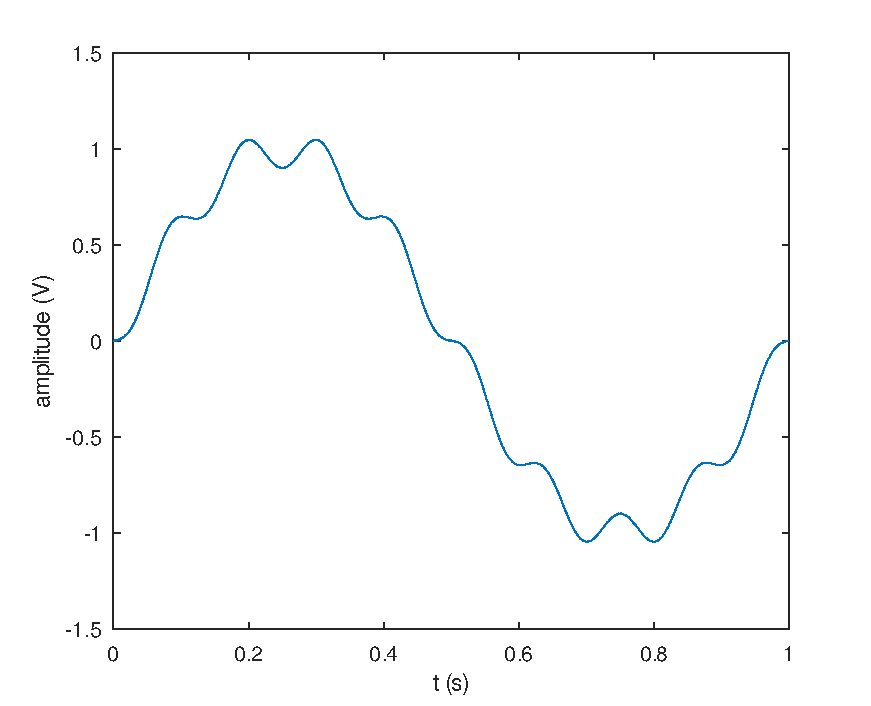
\includegraphics[width=0.7\textwidth]{algs_examples_published/GenNHarm_alg_example-1.pdf}
\end{center}


\phantomsection
\addcontentsline{toc}{section}{Generate simple sine waveform using number of periods}
\subsubsection*{Generate simple sine waveform using number of periods}



Consider we want to simulate 2.5 periods of a sine waveform.

\begin{lstlisting}
DI = [];
DI.fs.v = 1e3;
DI.M.v = 2.5;
DI.f.v = [1];
DI.A.v = [1];
DI.ph.v = [0];
DI.O.v = [0];
DI.noise.v = 0;
DO = qwtb('GenNHarm', DI);
figure
plot(DO.t.v, DO.y.v, '-');
xlabel('t (s)'), ylabel('amplitude (V)')
\end{lstlisting}
\begin{lstlisting}[language={},xleftmargin=5pt,frame=none]
QWTB: no uncertainty calculation
QWTB: GenNHarm wrapper: time series was calculated from sampling frequency and number of samples.
QWTB: GenNHarm wrapper: time series was calculated from number of main signal component periods.

\end{lstlisting}
\begin{center}
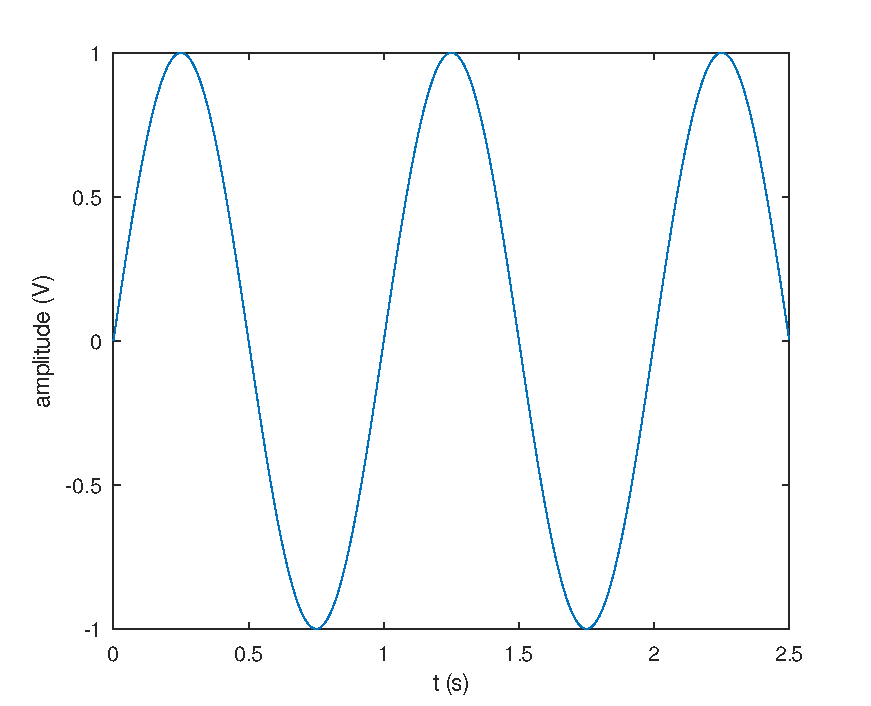
\includegraphics[width=0.7\textwidth]{algs_examples_published/GenNHarm_alg_example-2.pdf}
\end{center}


\phantomsection
\addcontentsline{toc}{section}{Generate waveform with automatically calculated harmonics}
\subsubsection*{Generate waveform with automatically calculated harmonics}



Consider waveform with 10 harmonic components, while the amplitudes of the
harmonics will be calculated based on the supplied THD\_k1 value. The \texttt{f},
\texttt{A}, \texttt{ph} and \texttt{O} quantities will contain only values for first harmonic. The
rest harmonics will be added by the waveform generator.

\begin{lstlisting}
DI = [];
DI.fs.v = 1e3;
DI.L.v = 1e3;
DI.f.v = [1];
DI.A.v = [1];
DI.ph.v = [0];
DI.O.v = [0];
DI.thd_k1.v = 0.1;
DI.nharm.v = 9;
DO = qwtb('GenNHarm', DI);
figure
plot(DO.t.v, DO.y.v, '-')
xlabel('t (s)'), ylabel('amplitude (V)')
\end{lstlisting}
\begin{lstlisting}[language={},xleftmargin=5pt,frame=none]
QWTB: no uncertainty calculation
QWTB: GenNHarm wrapper: time series was calculated from sampling frequency and number of samples.
QWTB: GenNHarm wrapper: time series was calculated from number of samples.

\end{lstlisting}
\begin{center}
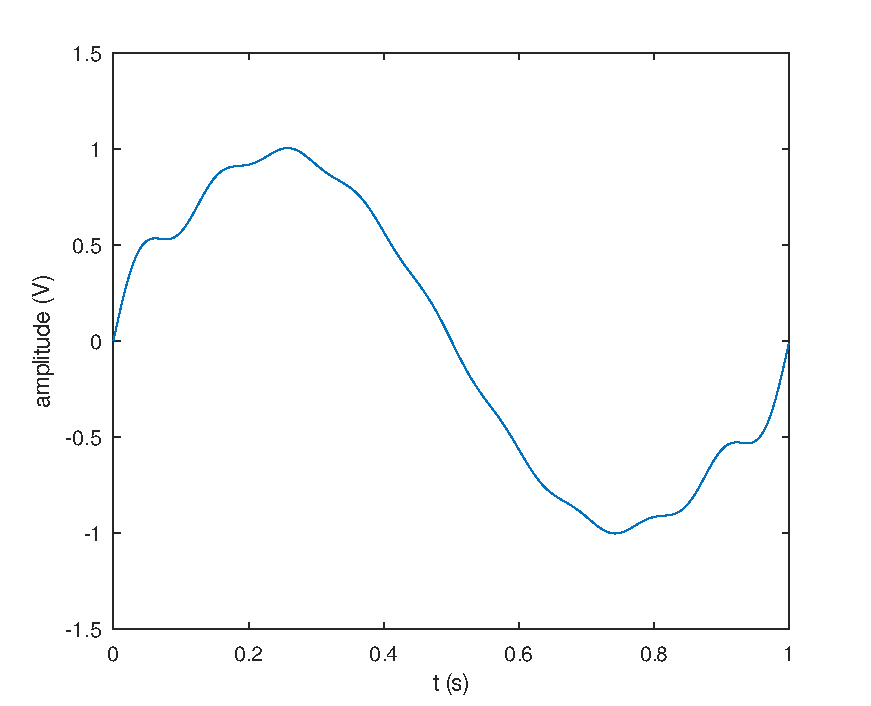
\includegraphics[width=0.7\textwidth]{algs_examples_published/GenNHarm_alg_example-3.pdf}
\end{center}


\phantomsection
\addcontentsline{toc}{section}{Check using FFT}
\subsubsection*{Check using FFT}



We can check the generated waveform by calculating the spectrum. Output of GenNHarm will be used as input into the algorithm \texttt{SP-WFFT}.

\begin{lstlisting}
DIspec = DO;
DIspec.fs.v = DI.fs.v;
DOspec = qwtb('SP-WFFT', DIspec);
figure
semilogy(DOspec.f.v, DOspec.A.v, 'o');
xlim([-2 12]); ylim([1e-3 10]);
\end{lstlisting}
\begin{lstlisting}[language={},xleftmargin=5pt,frame=none]
QWTB: no uncertainty calculation
warning: axis: omitting non-positive data in log plot
warning: called from
    __plt__>__plt2vv__ at line 502 column 10
    __plt__>__plt2__ at line 248 column 14
    __plt__ at line 115 column 16
    semilogy at line 65 column 10
    publish>eval_code_helper at line 1079 column 8
    publish>eval_code at line 995 column 30
    publish at line 402 column 9
    all_algs_examples2tex at line 51 column 5
 

\end{lstlisting}
\begin{center}
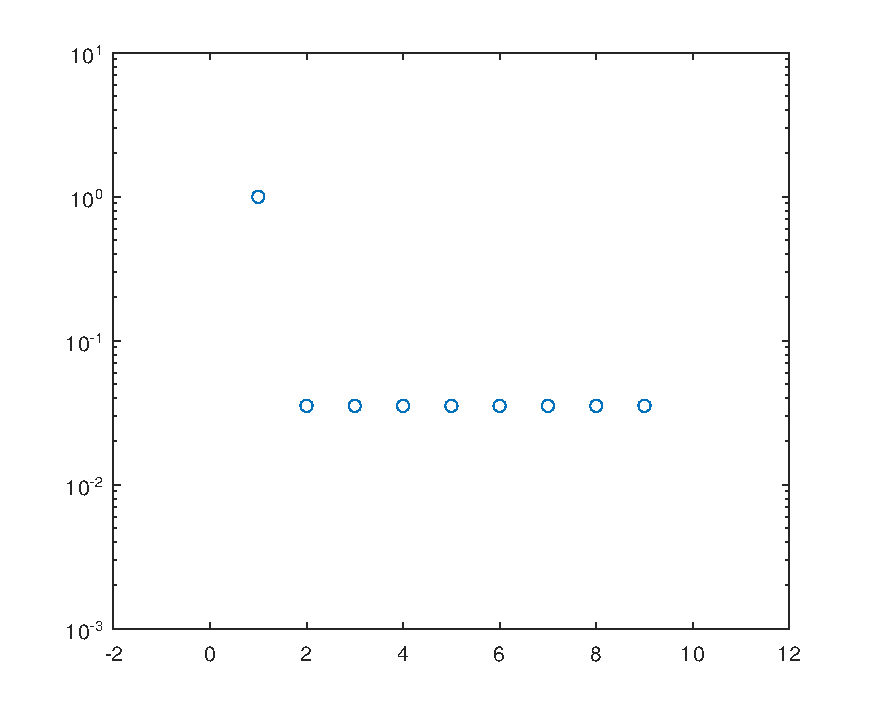
\includegraphics[width=0.7\textwidth]{algs_examples_published/GenNHarm_alg_example-4.pdf}
\end{center}


\stopcontents[localtoc]

\resumecontents[maintoc]

\chapter{iDFT2p -- 2-point interpolated DFT frequency estimator} %<<<1 ------------------------------
\chaptermark{iDFT2p}
\stopcontents[maintoc]
% included files are automatically generated by info_all_algs.m script and by Matlab publish
% function and converted by bash script betterpublish.
\section*{\infosection} %<<<2 -------------------
\begin{tightdesc}
\item [Id:] iDFT2p
\item [Name:] 2-point interpolated DFT frequency estimator
\item [Description:] An algorithm for estimating the frequency, amplitude, phase and offset of the fundamental component using interpolated discrete Fourier transform. Rectangular or Hann window can be used for DFT.
\item [Citation:] Krzysztof Duda: Interpolation algorithms of DFT for parameters estimation of sinusoidal and damped sinusoidal signals. In S. M. Salih, editor, Fourier Transform - Signal Processing, chapter 1, pages 3-32, InTech, 2012. \url{http://www.intechopen.com/books/fourier-transform-signal-processing/interpolated-dft} . Source code from: Rado Lapuh, "Sampling with 3458A, Understanding, Programming, Sampling and Signal Processing", ISBN 978-961-94476-0-4, 1st. ed., Ljubljana, Left Right d.o.o., 2018
\item [Remarks:] If sampling time |Ts| is not supplied, wrapper will calculate |Ts| from sampling frequency |fs| or if not supplied, mean of differences of time series |t| is used to calculate |Ts|. The optional parameter |window| can be set to values `rectangular` or `Hann`. If parameter is not supplied, Hann window will be used.
\item [License:] Implementation: MIT License
\item [Provides GUF:] no
\item [Provides MCM:] no
\item [Input Quantities] \rule{0em}{0em}
    \begin{tightdesc}
    \item [Required:] 
        \textsf{Ts} or \textsf{fs} or \textsf{t},\enspace \textsf{y}
    \item [Optional:] 
        \textsf{window}
    \item [Parameters:] 
        \textsf{window}
    \item [Descriptions:] \rule{0em}{0em}
        \begin{tightdesc}
            \item[\textsf{Ts}] -- Sampling time
            \item[\textsf{fs}] -- Sampling frequency
            \item[\textsf{t}] -- Time series
            \item[\textsf{window}] -- DFT window: `Hann` or `rectangular`
            \item[\textsf{y}] -- Sampled values
        \end{tightdesc}
    \end{tightdesc}
\item [Output Quantities:] \rule{0em}{0em}
    \begin{tightdesc}
        \item[\textsf{A}] -- Amplitude of main signal component
        \item[\textsf{O}] -- Offset of main signal component
        \item[\textsf{f}] -- Frequency of main signal component
        \item[\textsf{ph}] -- Phase of main signal component
    \end{tightdesc}
\end{tightdesc}

\section*{\examplesection} %<<<2 ------------------------
\startcontents[localtoc]
\printcontents[localtoc]{}{0}{\subsection*{Contents}\setcounter{tocdepth}{2}}



\phantomsection
\addcontentsline{toc}{section}{Generate sample data}
\subsubsection*{Generate sample data}



Two quantities are prepared: \texttt{Ts} and \texttt{y}, representing 0.5 second of sinus waveform of nominal
frequency 100 Hz, nominal amplitude 1 V and nominal phase 1 rad, sampled with sampling time 0.1
ms, with offset 0.1 V. The sampling is not coherent.

\begin{lstlisting}
DI = [];
Anom = 1; fnom = 100; phnom = 1; Onom = 0.1;
DI.Ts.v = 1e-4;
t = [0:DI.Ts.v:0.5];
DI.y.v = Anom*sin(2*pi*fnom*t + phnom) + Onom;
\end{lstlisting}


\phantomsection
\addcontentsline{toc}{section}{Call algorithm}
\subsubsection*{Call algorithm}



First a rectangular window will be selected to estimate main signal properties. Use QWTB to apply
algorithm \texttt{iDFT3p} to data \texttt{DI} and put results into \texttt{DOr}.

\begin{lstlisting}
DI.window.v = 'rectangular';
DOr = qwtb('iDFT2p', DI);
\end{lstlisting}
\begin{lstlisting}[language={},xleftmargin=5pt,frame=none]
QWTB: no uncertainty calculation

\end{lstlisting}


Next a Hann window will be selected to estimate main signal properties Results will be put into \texttt{DOh}.

\begin{lstlisting}
DI.window.v = 'Hann';
DOh = qwtb('iDFT2p', DI);
\end{lstlisting}
\begin{lstlisting}[language={},xleftmargin=5pt,frame=none]
QWTB: no uncertainty calculation

\end{lstlisting}


\phantomsection
\addcontentsline{toc}{section}{Display results}
\subsubsection*{Display results}



Results is the amplitude, frequency and phase of sampled waveform. For rectangular window, the
error from nominal in parts per milion is:

\begin{lstlisting}
f_re = (DOr.f.v - fnom)./fnom .* 1e6
A_re = (DOr.A.v - Anom)./Anom .* 1e6
ph_re = (DOr.ph.v - phnom)./phnom .* 1e6
O_re = (DOr.O.v - Onom)./Onom .* 1e6
\end{lstlisting}
\begin{lstlisting}[language={},xleftmargin=5pt,frame=none]
f_re = -0.8083
A_re = 40.315
ph_re = 217.94
O_re = 1682.6

\end{lstlisting}


For Hann window:

\begin{lstlisting}
f_he = (DOh.f.v - fnom)./fnom .* 1e6
A_he = (DOh.A.v - Anom)./Anom .* 1e6
ph_he = (DOh.ph.v - phnom)./phnom .* 1e6
O_he = (DOh.O.v - Onom)./Onom .* 1e6
\end{lstlisting}
\begin{lstlisting}[language={},xleftmargin=5pt,frame=none]
f_he = 1.8426e-04
A_he = -4.6039e-03
ph_he = 6.2442
O_he = -0.6862

\end{lstlisting}


\stopcontents[localtoc]

\resumecontents[maintoc]

\chapter{iDFT3p -- 3-point interpolated DFT frequency estimator} %<<<1 ------------------------------
\chaptermark{iDFT3p}
\stopcontents[maintoc]
% included files are automatically generated by info_all_algs.m script and by Matlab publish
% function and converted by bash script betterpublish.
\section*{\infosection} %<<<2 -------------------
\begin{tightdesc}
\item [Id:] iDFT3p
\item [Name:] 3-point interpolated DFT frequency estimator
\item [Description:] An algorithm for estimating the frequency, amplitude, phase and offset of the fundamental component using interpolated discrete Fourier transform. Rectangular or Hann window can be used for DFT.
\item [Citation:] Krzysztof Duda: Interpolation algorithms of DFT for parameters estimation of sinusoidal and damped sinusoidal signals. In S. M. Salih, editor, Fourier Transform - Signal Processing, chapter 1, pages 3-32, InTech, 2012. \url{http://www.intechopen.com/books/fourier-transform-signal-processing/interpolated-dft} . Source code from: Rado Lapuh, "Sampling with 3458A, Understanding, Programming, Sampling and Signal Processing", ISBN 978-961-94476-0-4, 1st. ed., Ljubljana, Left Right d.o.o., 2018
\item [Remarks:] If sampling time |Ts| is not supplied, wrapper will calculate |Ts| from sampling frequency |fs| or if not supplied, mean of differences of time series |t| is used to calculate |Ts|. The optional parameter |window| can be set to values `rectangular` or `Hann`. If parameter is not supplied, Hann window will be used.
\item [License:] Implementation: MIT License
\item [Provides GUF:] no
\item [Provides MCM:] no
\item [Input Quantities] \rule{0em}{0em}
    \begin{tightdesc}
    \item [Required:] 
        \textsf{Ts} or \textsf{fs} or \textsf{t},\enspace \textsf{y}
    \item [Optional:] 
        \textsf{window}
    \item [Parameters:] 
        \textsf{window}
    \item [Descriptions:] \rule{0em}{0em}
        \begin{tightdesc}
            \item[\textsf{Ts}] -- Sampling time
            \item[\textsf{fs}] -- Sampling frequency
            \item[\textsf{t}] -- Time series
            \item[\textsf{window}] -- DFT window: `Hann` or `rectangular`
            \item[\textsf{y}] -- Sampled values
        \end{tightdesc}
    \end{tightdesc}
\item [Output Quantities:] \rule{0em}{0em}
    \begin{tightdesc}
        \item[\textsf{A}] -- Amplitude of main signal component
        \item[\textsf{O}] -- Offset of main signal component
        \item[\textsf{f}] -- Frequency of main signal component
        \item[\textsf{ph}] -- Phase of main signal component
    \end{tightdesc}
\end{tightdesc}

\section*{\examplesection} %<<<2 ------------------------
\startcontents[localtoc]
\printcontents[localtoc]{}{0}{\subsection*{Contents}\setcounter{tocdepth}{2}}



\phantomsection
\addcontentsline{toc}{section}{Generate sample data}
\subsubsection*{Generate sample data}



Two quantities are prepared: \texttt{Ts} and \texttt{y}, representing 0.5 second of sinus waveform of nominal
frequency 100 Hz, nominal amplitude 1 V and nominal phase 1 rad, sampled with sampling time 0.1
ms, with offset 0.1 V. The sampling is not coherent.

\begin{lstlisting}
DI = [];
Anom = 1; fnom = 100; phnom = 1; Onom = 0.1;
DI.Ts.v = 1e-4;
t = [0:DI.Ts.v:0.5];
DI.y.v = Anom*sin(2*pi*fnom*t + phnom) + Onom;
\end{lstlisting}


\phantomsection
\addcontentsline{toc}{section}{Call algorithm}
\subsubsection*{Call algorithm}



First a rectangular window will be selected to estimate main signal properties. Use QWTB to apply
algorithm \texttt{iDFT3p} to data \texttt{DI} and put results into \texttt{DOr}.

\begin{lstlisting}
DI.window.v = 'rectangular';
DOr = qwtb('iDFT3p', DI);
\end{lstlisting}
\begin{lstlisting}[language={},xleftmargin=5pt,frame=none]
QWTB: no uncertainty calculation

\end{lstlisting}


Next a Hann window will be selected to estimate main signal properties Results will be put into \texttt{DOh}.

\begin{lstlisting}
DI.window.v = 'Hann';
DOh = qwtb('iDFT3p', DI);
\end{lstlisting}
\begin{lstlisting}[language={},xleftmargin=5pt,frame=none]
QWTB: no uncertainty calculation

\end{lstlisting}


\phantomsection
\addcontentsline{toc}{section}{Display results}
\subsubsection*{Display results}



Results is the amplitude, frequency and phase of sampled waveform. For rectangular window, the
error from nominal in parts per milion is:

\begin{lstlisting}
f_re = (DOr.f.v - fnom)./fnom .* 1e6
A_re = (DOr.A.v - Anom)./Anom .* 1e6
ph_re = (DOr.ph.v - phnom)./phnom .* 1e6
O_re = (DOr.O.v - Onom)./Onom .* 1e6
\end{lstlisting}
\begin{lstlisting}[language={},xleftmargin=5pt,frame=none]
f_re = 0.016607
A_re = 41.257
ph_re = 88.368
O_re = 1682.6

\end{lstlisting}


For Hann window:

\begin{lstlisting}
f_he = (DOh.f.v - fnom)./fnom .* 1e6
A_he = (DOh.A.v - Anom)./Anom .* 1e6
ph_he = (DOh.ph.v - phnom)./phnom .* 1e6
O_he = (DOh.O.v - Onom)./Onom .* 1e6
\end{lstlisting}
\begin{lstlisting}[language={},xleftmargin=5pt,frame=none]
f_he = -3.7790e-06
A_he = 3.9702e-07
ph_he = 6.2737
O_he = -0.6862

\end{lstlisting}


\stopcontents[localtoc]

\resumecontents[maintoc]

\chapter{INL-DNL -- Integral and Differential Non-Linearity of ADC} %<<<1 ------------------------------
\chaptermark{INL-DNL}
\stopcontents[maintoc]
% included files are automatically generated by info_all_algs.m script and by Matlab publish
% function and converted by bash script betterpublish.
\section*{\infosection} %<<<2 -------------------
\input{algs_info_published/info_INL-DNL.tex}
\section*{\examplesection} %<<<2 ------------------------
\startcontents[localtoc]
\printcontents[localtoc]{}{0}{\subsection*{Contents}\setcounter{tocdepth}{2}}



\phantomsection
\addcontentsline{toc}{section}{Generate sample data}
\subsubsection*{Generate sample data}



Suppose a sine wave of nominal frequency 10 Hz and nominal amplitude 1.5 V is sampled by ADC with
bit resolution of 4 and full range of 1 V. First quantity \texttt{bitres} with number of bits of
resolution of the ADC is prepared and put into input data structure \texttt{DI}.

\begin{lstlisting}
DI = [];
DI.bitres.v = 4;
\end{lstlisting}


Waveform is constructed. Amplitude is selected to overload the ADC.

\begin{lstlisting}
t=[0:1/1e4:1-1/1e4];
Anom = 3.5; fnom = 2; phnom = 0;
wvfrm = Anom*sin(2*pi*fnom*t + phnom);
\end{lstlisting}


Next ADC code values are calculated. It is simulated by quantization and scaling of the sampled
waveform. In real measurement code values can be obtained directly from the ADC. Suppose ADC range
is -2..2.

\begin{lstlisting}
codes = wvfrm;
rmin = -2; rmax = 2;
levels = 2.^DI.bitres.v - 1;
codes(codes<rmin) = rmin;
codes(codes>rmax) = rmax;
codes = round((codes-rmin)./(rmax-rmin).*levels);
\end{lstlisting}


Now lets introduce ADC error. Instead of generating code 2 ADC erroneously generates
code 3 and instead of 11 it generates 10.

\begin{lstlisting}
codes(codes==2) = 3;
codes(codes==11) = 10;
codes = codes + min(codes);
\end{lstlisting}


Create quantity \texttt{codes} and plot a figure with sampled sine wave and codes.

\begin{lstlisting}
DI.codes.v = codes;
figure
hold on
stairs(t, codes);
wvfrm = (wvfrm - rmin)./(rmax-rmin).*levels;
plot(t, wvfrm, '-r');
xlabel('t (s)')
ylabel('Codes / Voltage (scaled)');
legend('Codes generated by ADC','Original waveform scaled to match codes');
hold off
\end{lstlisting}
\begin{center}
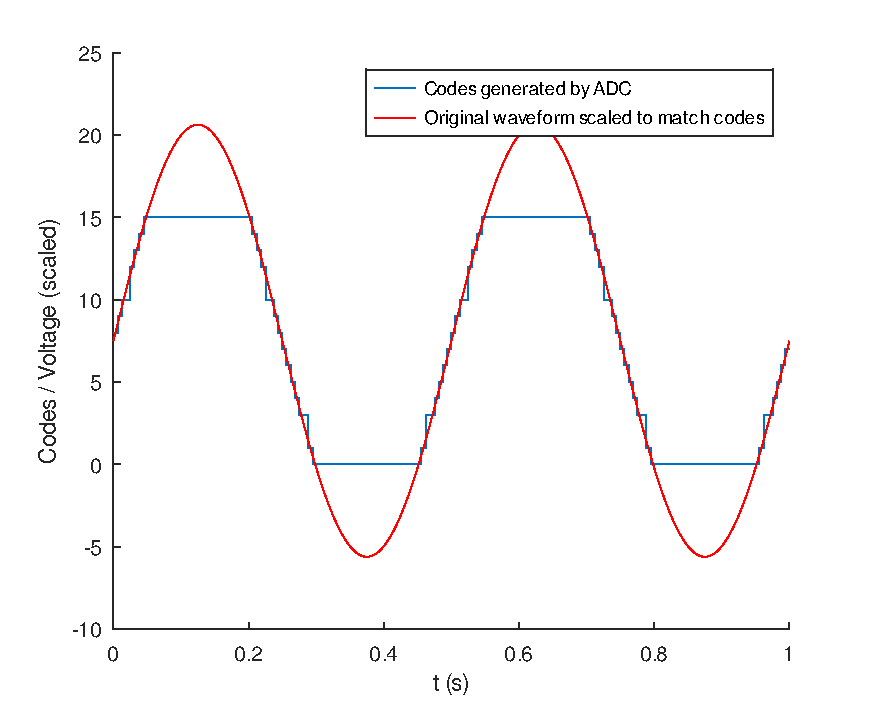
\includegraphics[width=0.7\textwidth]{algs_examples_published/INL-DNL_alg_example-1.pdf}
\end{center}


\phantomsection
\addcontentsline{toc}{section}{Call algorithm}
\subsubsection*{Call algorithm}



Apply INL algorithm to the input data \texttt{DI}.

\begin{lstlisting}
DO = qwtb('INL-DNL', DI);
\end{lstlisting}
\begin{lstlisting}[language={},xleftmargin=5pt,frame=none]
QWTB: no uncertainty calculation
warning: Invalid UTF-8 byte sequences have been replaced.
warning: called from
    ProcessHistogramTest at line 52 column 3
    alg_wrapper at line 35 column 5
    qwtb>check_and_run_alg at line 377 column 17
    qwtb at line 114 column 47
    publish>eval_code_helper at line 1079 column 8
    publish>eval_code at line 995 column 30
    publish at line 402 column 9
    all_algs_examples2tex at line 51 column 5
 
warning: Invalid UTF-8 byte sequences have been replaced.
warning: called from
    ProcessHistogramTest at line 273 column 14
    alg_wrapper at line 35 column 5
    qwtb>check_and_run_alg at line 377 column 17
    qwtb at line 114 column 47
    publish>eval_code_helper at line 1079 column 8
    publish>eval_code at line 995 column 30
    publish at line 402 column 9
    all_algs_examples2tex at line 51 column 5
 

\end{lstlisting}


Plot results of integral non-linearity. One can clearly observe defects on codes 3 and
11.

\begin{lstlisting}
figure
plot(DO.INL.v, '-x');
xlabel('Transition levels')
ylabel('INL (k)')
\end{lstlisting}
\begin{center}
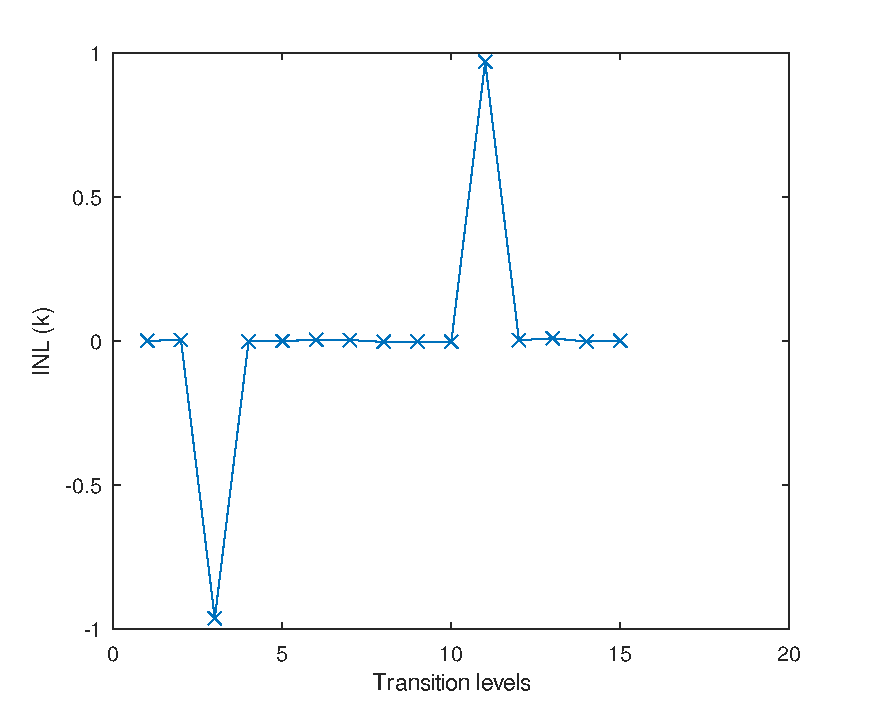
\includegraphics[width=0.7\textwidth]{algs_examples_published/INL-DNL_alg_example-2.pdf}
\end{center}


Plot results of differential non-linearity. One can clearly observe defects on transitions 2-3 and
10-11.

\begin{lstlisting}
figure
plot(DO.DNL.v, '-x');
xlabel('Code bins')
ylabel('DNL (k)')
\end{lstlisting}
\begin{center}
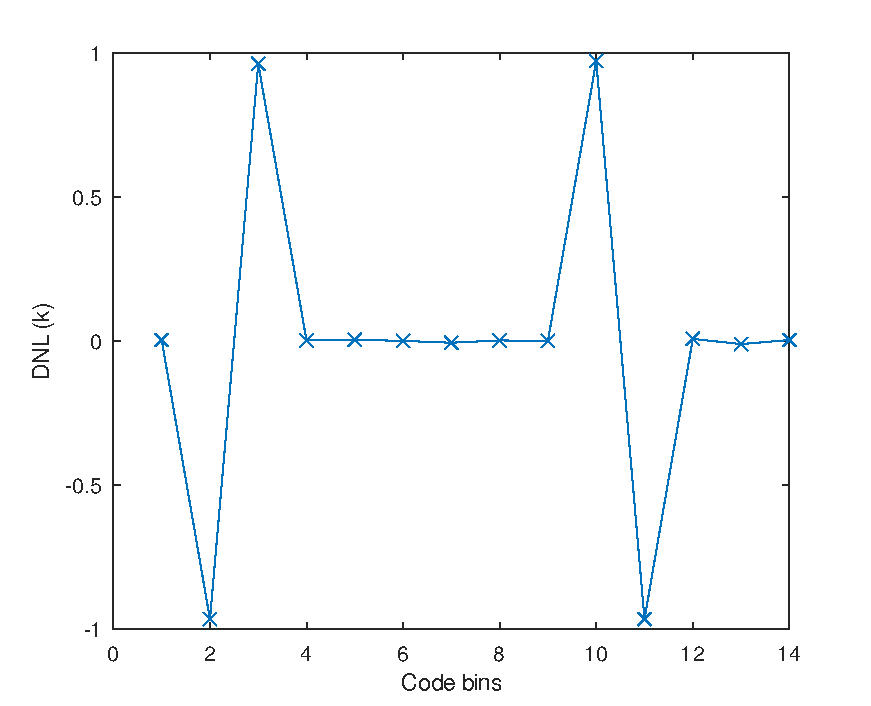
\includegraphics[width=0.7\textwidth]{algs_examples_published/INL-DNL_alg_example-3.pdf}
\end{center}


\stopcontents[localtoc]

\resumecontents[maintoc]

\chapter{ISOTS28037 -- NPL’s Software to Support ISO/TS 28037:2010(E)} %<<<1 ------------------------------
\chaptermark{ISOTS28037}
\stopcontents[maintoc]
% included files are automatically generated by info_all_algs.m script and by Matlab publish
% function and converted by bash script betterpublish.
\section*{\infosection} %<<<2 -------------------
\begin{tightdesc}
\item [Id:] ISOTS28037
\item [Name:] NPL’s Software to Support ISO/TS 28037:2010(E)
\item [Description:] NPL’s Software to Support ISO/TS 28037:2010(E) software implements the algorithms described in the ISO Technical Specification "Determination and use of straight-line calibration functions" and has been developed by the National Physical Laboratory (NPL) in the United Kingdom. The software is available as a compressed ZIP folder from the web sites of NPL at www.npl.co.uk/mathematics-scientific-computing/software-support-for-metrology/software-downloads-(ssfm) and the International Organization for Standardization at standards.iso.org/iso/ts/28037/. Downloadable at https://www.npl.co.uk/resources/software/iso-ts-28037-2010e
\item [Citation:] \url{https://standards.iso.org/iso/ts/28037/,} \url{https://www.npl.co.uk/resources/software/iso-ts-28037-2010e}
\item [Remarks:] Implements methods WSL, GDR. GMR nor GGMR are not implemented.
\item [License:] NPL license
\item [Provides GUF:] yes
\item [Provides MCM:] no
\item [Input Quantities] \rule{0em}{0em}
    \begin{tightdesc}
    \item [Required:] 
        \textsf{x},\enspace \textsf{y}
    \item [Optional:] 
        \textsf{tol},\enspace \textsf{xhat}
    \item [Parameters:] 
        \textsf{tol}
    \item [Descriptions:] \rule{0em}{0em}
        \begin{tightdesc}
            \item[\textsf{tol}] -- Tolerance for convergence of iterative method GDR. Iterations stops when increments of parameters a, b is smaller than tol*norm([a b]).
            \item[\textsf{x}] -- Independent variable
            \item[\textsf{xhat}] -- Independent variable values to be (extra/inter)polated (forward evaluated).
            \item[\textsf{y}] -- Dependent variable
        \end{tightdesc}
    \end{tightdesc}
\item [Output Quantities:] \rule{0em}{0em}
    \begin{tightdesc}
        \item[\textsf{chisq}] -- 95 % quantile of chi-squared distribution
        \item[\textsf{coefs}] -- Fitted coefficients
        \item[\textsf{exponents}] -- Exponents of polynomial used to fit, for now only [0 1] possible
        \item[\textsf{func}] -- Inline function constructed for exponents with parameters `x` and `coefs.v`
        \item[\textsf{model}] -- Model used for calculation.
        \item[\textsf{model\_rejected}] -- If 1, straight-line model is rejected. Estimated as chi\_sq\_obs > chi\_sq.
        \item[\textsf{yhat}] -- Fitted values y
    \end{tightdesc}
\end{tightdesc}

\section*{\examplesection} %<<<2 ------------------------
\startcontents[localtoc]
\printcontents[localtoc]{}{0}{\subsection*{Contents}\setcounter{tocdepth}{2}}

\begin{lstlisting}
% Example for algorithm ISOTS28037
\end{lstlisting}


\phantomsection
\addcontentsline{toc}{section}{Generate sample data}
\subsubsection*{Generate sample data}



Set independent and dependent variables.

\begin{lstlisting}
DI.x.v = [1 2 3 4 5];
DI.x.u = [0.1 0.1 0.1 0.1 0.1];
DI.y.v = [1.1 1.9 3.1 3.9 5.1];
DI.y.u = [0.1 0.1 0.1 0.1 0.1];

% Set values for interpolation:
DI.xhat.v = [0:0.1:6];
DI.xhat.u = 0.1 + zeros(size(DI.xhat.v));
\end{lstlisting}


\phantomsection
\addcontentsline{toc}{section}{Call algorithm}
\subsubsection*{Call algorithm}



Use QWTB to apply algorithm \texttt{ISOTS28037} to data \texttt{DI}.

\begin{lstlisting}
DO = qwtb('ISOTS28037', DI);
\end{lstlisting}
\begin{lstlisting}[language={},xleftmargin=5pt,frame=none]
QWTB: no uncertainty calculation

\end{lstlisting}


\phantomsection
\addcontentsline{toc}{section}{Display results}
\subsubsection*{Display results}



Results is

\begin{lstlisting}
disp(['offset          : ' num2str(DO.coefs.v(1)) ' +- ' num2str(DO.coefs.u(1))])
disp(['linear coeff.   : ' num2str(DO.coefs.v(2)) ' +- ' num2str(DO.coefs.u(2))])
\end{lstlisting}
\begin{lstlisting}[language={},xleftmargin=5pt,frame=none]
offset          : 1.0024 +- 0.044802
linear coeff.   : 0.012791 +- 0.14858

\end{lstlisting}


\phantomsection
\addcontentsline{toc}{section}{Plot results}
\subsubsection*{Plot results}

\begin{lstlisting}
figure
hold on
errorbar(DI.x.v, DI.y.v, DI.x.u, DI.x.u, DI.y.u, DI.y.u, '~>xb')
plot(DI.xhat.v, DO.yhat.v, 'r-')
plot(DI.xhat.v, DO.yhat.v + DI.xhat.u, 'k-')
plot(DI.xhat.v, DO.yhat.v - DI.xhat.u, 'k-')
xlabel('independent variable')
ylabel('dependent variable')
legend('original data','fit', 'interpolated values', 'uncer. of int. val.','location','southeast')
hold off
\end{lstlisting}
\begin{center}
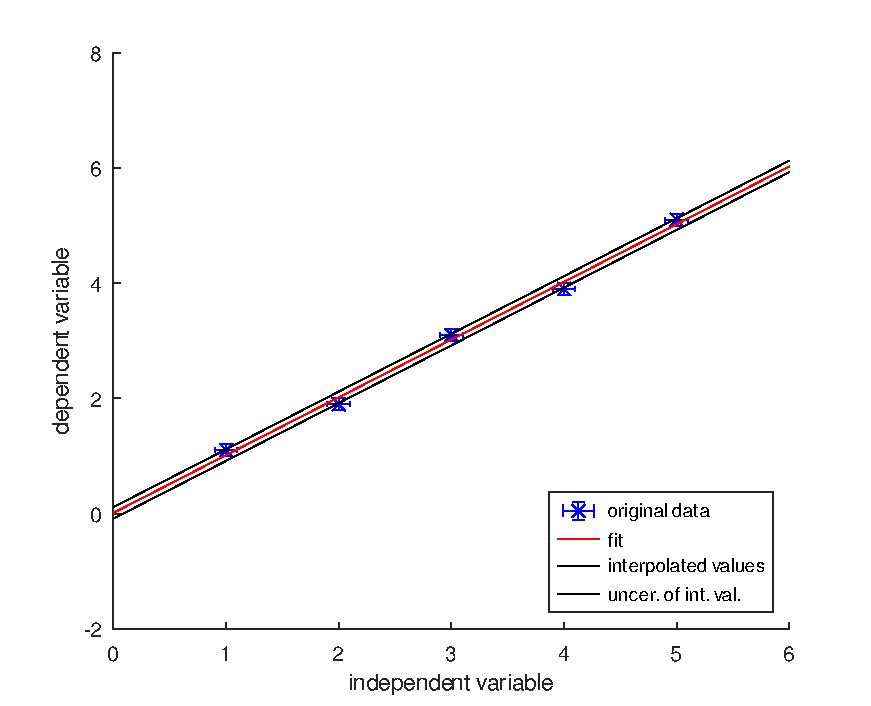
\includegraphics[width=0.7\textwidth]{algs_examples_published/ISOTS28037_alg_example-1.pdf}
\end{center}


\stopcontents[localtoc]

\resumecontents[maintoc]

\chapter{MADEV -- Modified Allan Deviation} %<<<1 ------------------------------
\chaptermark{MADEV}
\stopcontents[maintoc]
% included files are automatically generated by info_all_algs.m script and by Matlab publish
% function and converted by bash script betterpublish.
\section*{\infosection} %<<<2 -------------------
\input{algs_info_published/info_MADEV.tex}
\section*{\examplesection} %<<<2 ------------------------
\startcontents[localtoc]
\printcontents[localtoc]{}{0}{\subsection*{Contents}\setcounter{tocdepth}{2}}



\phantomsection
\addcontentsline{toc}{section}{Generate sample data}
\subsubsection*{Generate sample data}



A random numbers with normal probability distribution function will be generated into input data \texttt{DI.y.v}. Next a drift will be added.

\begin{lstlisting}
DI = [];
DI.y.v = 1.5 + 3.*randn(1, 1e3);
DI.y.v = DI.y.v + [1:1:1e3]./100;
\end{lstlisting}


Lets suppose a sampling frequency is 1 Hz. The algorithm will generate all possible tau values automatically.

\begin{lstlisting}
DI.fs.v = 1;
\end{lstlisting}


\phantomsection
\addcontentsline{toc}{section}{Call algorithm}
\subsubsection*{Call algorithm}



Use QWTB to apply algorithm \texttt{MADEV} to data \texttt{DI}.

\begin{lstlisting}
DO = qwtb('MADEV', DI);
\end{lstlisting}
\begin{lstlisting}[language={},xleftmargin=5pt,frame=none]
QWTB: no uncertainty calculation

\end{lstlisting}


\phantomsection
\addcontentsline{toc}{section}{Display results}
\subsubsection*{Display results}



Log log figure is the best to see modified allan deviation results:

\begin{lstlisting}
figure; hold on
loglog(DO.tau.v, DO.madev.v, '-b')
loglog(DO.tau.v, DO.madev.v + DO.madev.u, '-k')
loglog(DO.tau.v, DO.madev.v - DO.madev.u, '-k')
xlabel('\tau (sec)');
ylabel('\sigma_y(\tau)');
title(['period = ' num2str(DI.fs.v)]);
grid('on'); hold off
\end{lstlisting}
\begin{lstlisting}[language={},xleftmargin=5pt,frame=none]
warning: axis: omitting non-positive data in log plot
warning: called from
    __plt__>__plt2vv__ at line 502 column 10
    __plt__>__plt2__ at line 248 column 14
    __plt__ at line 115 column 16
    loglog at line 65 column 10
    publish>eval_code_helper at line 1079 column 8
    publish>eval_code at line 995 column 30
    publish at line 402 column 9
    all_algs_examples2tex at line 51 column 5
 
warning: axis: omitting non-positive data in log plot
warning: called from
    __plt__>__plt2vv__ at line 502 column 10
    __plt__>__plt2__ at line 248 column 14
    __plt__ at line 115 column 16
    loglog at line 65 column 10
    publish>eval_code_helper at line 1079 column 8
    publish>eval_code at line 995 column 30
    publish at line 402 column 9
    all_algs_examples2tex at line 51 column 5
 
warning: axis: omitting non-positive data in log plot
warning: called from
    __plt__>__plt2vv__ at line 502 column 10
    __plt__>__plt2__ at line 248 column 14
    __plt__ at line 115 column 16
    loglog at line 65 column 10
    publish>eval_code_helper at line 1079 column 8
    publish>eval_code at line 995 column 30
    publish at line 402 column 9
    all_algs_examples2tex at line 51 column 5
 
warning: axis: omitting non-positive data in log plot
warning: called from
    __plt__>__plt2vv__ at line 502 column 10
    __plt__>__plt2__ at line 248 column 14
    __plt__ at line 115 column 16
    loglog at line 65 column 10
    publish>eval_code_helper at line 1079 column 8
    publish>eval_code at line 995 column 30
    publish at line 402 column 9
    all_algs_examples2tex at line 51 column 5
 
warning: axis: omitting non-positive data in log plot
warning: called from
    __plt__>__plt2vv__ at line 502 column 10
    __plt__>__plt2__ at line 248 column 14
    __plt__ at line 115 column 16
    loglog at line 65 column 10
    publish>eval_code_helper at line 1079 column 8
    publish>eval_code at line 995 column 30
    publish at line 402 column 9
    all_algs_examples2tex at line 51 column 5
 

\end{lstlisting}
\begin{center}
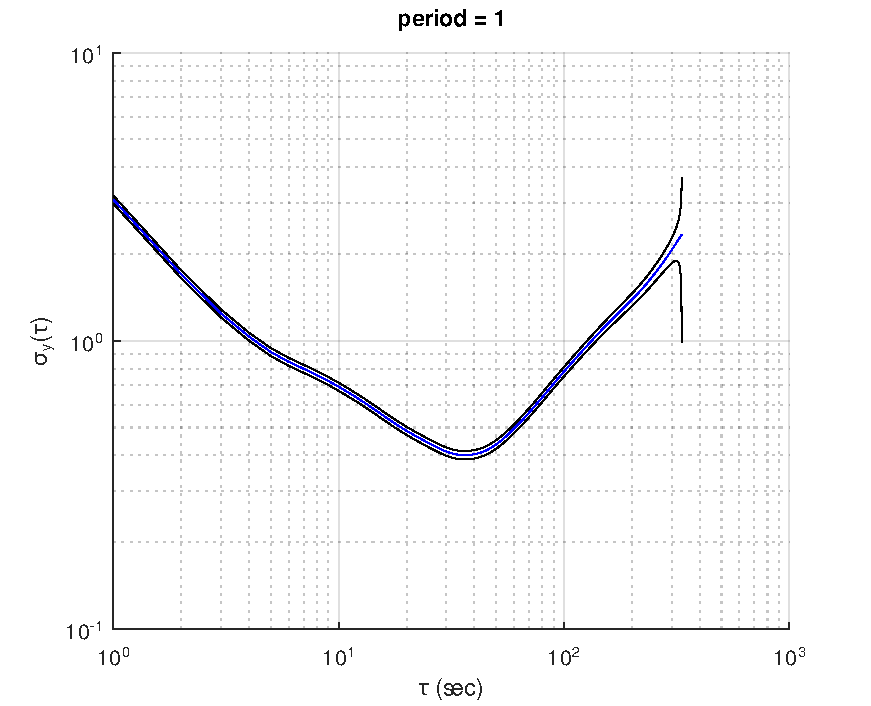
\includegraphics[width=0.7\textwidth]{algs_examples_published/MADEV_alg_example-1.pdf}
\end{center}


\stopcontents[localtoc]

\resumecontents[maintoc]

\chapter{OADEV -- Overlapping Allan Deviation} %<<<1 ------------------------------
\chaptermark{OADEV}
\stopcontents[maintoc]
% included files are automatically generated by info_all_algs.m script and by Matlab publish
% function and converted by bash script betterpublish.
\section*{\infosection} %<<<2 -------------------
\input{algs_info_published/info_OADEV.tex}
\section*{\examplesection} %<<<2 ------------------------
\startcontents[localtoc]
\printcontents[localtoc]{}{0}{\subsection*{Contents}\setcounter{tocdepth}{2}}



\phantomsection
\addcontentsline{toc}{section}{Generate sample data}
\subsubsection*{Generate sample data}



A random numbers with normal probability distribution function will be generated into input data \texttt{DI.y.v}. Next a drift will be added.

\begin{lstlisting}
DI = [];
DI.y.v = 1.5 + 3.*randn(1, 1e3);
DI.y.v = DI.y.v + [1:1:1e3]./100;
\end{lstlisting}


Lets suppose a sampling frequency is 1 Hz. The algorithm will generate all possible tau values automatically.

\begin{lstlisting}
DI.fs.v = 1;
\end{lstlisting}


\phantomsection
\addcontentsline{toc}{section}{Call algorithm}
\subsubsection*{Call algorithm}



Use QWTB to apply algorithm \texttt{OADEV} to data \texttt{DI}.

\begin{lstlisting}
DO = qwtb('OADEV', DI);
\end{lstlisting}
\begin{lstlisting}[language={},xleftmargin=5pt,frame=none]
QWTB: no uncertainty calculation

\end{lstlisting}


\phantomsection
\addcontentsline{toc}{section}{Display results}
\subsubsection*{Display results}



Log log figure is the best to see allan deviation results:

\begin{lstlisting}
figure; hold on
loglog(DO.tau.v, DO.oadev.v, '-b')
loglog(DO.tau.v, DO.oadev.v + DO.oadev.u, '-k')
loglog(DO.tau.v, DO.oadev.v - DO.oadev.u, '-k')
xlabel('\tau (sec)');
ylabel('\sigma_y(\tau)');
title(['period = ' num2str(DI.fs.v)]);
grid('on'); hold off
\end{lstlisting}
\begin{lstlisting}[language={},xleftmargin=5pt,frame=none]
warning: axis: omitting non-positive data in log plot
warning: called from
    __plt__>__plt2vv__ at line 502 column 10
    __plt__>__plt2__ at line 248 column 14
    __plt__ at line 115 column 16
    loglog at line 65 column 10
    publish>eval_code_helper at line 1079 column 8
    publish>eval_code at line 995 column 30
    publish at line 402 column 9
    all_algs_examples2tex at line 51 column 5
 

\end{lstlisting}
\begin{center}
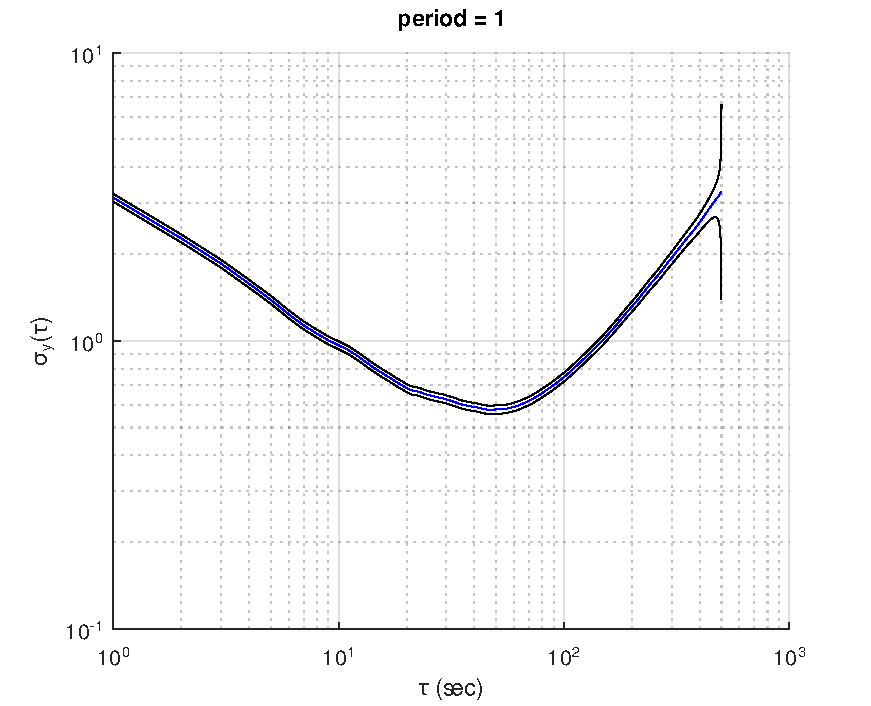
\includegraphics[width=0.7\textwidth]{algs_examples_published/OADEV_alg_example-1.pdf}
\end{center}


\stopcontents[localtoc]

\resumecontents[maintoc]

\chapter{PSFE -- Phase Sensitive Frequency Estimator} %<<<1 ------------------------------
\chaptermark{PSFE}
\stopcontents[maintoc]
% included files are automatically generated by info_all_algs.m script and by Matlab publish
% function and converted by bash script betterpublish.
\section*{\infosection} %<<<2 -------------------
\begin{tightdesc}
\item [Id:] PSFE
\item [Name:] Phase Sensitive Frequency Estimator
\item [Description:] An algorithm for estimating the frequency, amplitude, and phase of the fundamental component in harmonically distorted waveforms. The algorithm minimizes the phase difference between the sine model and the sampled waveform by effectively minimizing the influence of the harmonic components. It uses a three-parameter sine-fitting algorithm for all phase calculations. The resulting estimates show up to two orders of magnitude smaller sensitivity to harmonic distortions than the results of the four-parameter sine fitting algorithm. PSFE requires more than two periods of sampled signal and at least 6 samples in the Record.
\item [Citation:] Lapuh, R., "Estimating the Fundamental Component of Harmonically Distorted Signals From Noncoherently Sampled Data," Instrumentation and Measurement, IEEE Transactions on , vol.64, no.6, pp.1419,1424, June 2015, doi: 10.1109/TIM.2015.2401211, URL: \url{http://ieeexplore.ieee.org/stamp/stamp.jsp?tp=\&arnumber=7061456\&isnumber=7104190.} Source code from: Rado Lapuh, "Sampling with 3458A, Understanding, Programming, Sampling and Signal Processing", ISBN 978-961-94476-0-4, 1st. ed., Ljubljana, Left Right d.o.o., 2018
\item [Remarks:] If sampling time |Ts| is not supplied, wrapper will calculate |Ts| from sampling frequency |fs| or if not supplied, mean of differences of time series |t| is used to calculate |Ts|.
\item [License:] MIT License
\item [Provides GUF:] no
\item [Provides MCM:] no
\item [Input Quantities] \rule{0em}{0em}
    \begin{tightdesc}
    \item [Required:] 
        \textsf{Ts} or \textsf{fs} or \textsf{t},\enspace \textsf{y}
    \item [Descriptions:] \rule{0em}{0em}
        \begin{tightdesc}
            \item[\textsf{Ts}] -- Sampling time
            \item[\textsf{fs}] -- Sampling frequency
            \item[\textsf{t}] -- Time series
            \item[\textsf{y}] -- Sampled values
        \end{tightdesc}
    \end{tightdesc}
\item [Output Quantities:] \rule{0em}{0em}
    \begin{tightdesc}
        \item[\textsf{A}] -- Amplitude of main signal component
        \item[\textsf{O}] -- Offset of main signal component
        \item[\textsf{f}] -- Frequency of main signal component
        \item[\textsf{ph}] -- Phase of main signal component
    \end{tightdesc}
\end{tightdesc}

\section*{\examplesection} %<<<2 ------------------------
\startcontents[localtoc]
\printcontents[localtoc]{}{0}{\subsection*{Contents}\setcounter{tocdepth}{2}}



\phantomsection
\addcontentsline{toc}{section}{Generate sample data}
\subsubsection*{Generate sample data}



Two quantities are prepared: \texttt{Ts} and \texttt{y}, representing 1 second of sinus
waveform of nominal frequency 100 Hz, nominal amplitude 1 V and nominal phase
1 rad, sampled with sampling time 0.1 ms.

\begin{lstlisting}
DI = [];
Anom = 1; fnom = 100; phnom = 1;
DI.Ts.v = 1e-4;
t = [0:DI.Ts.v:1-DI.Ts.v];
DI.y.v = Anom*sin(2*pi*fnom*t + phnom);
\end{lstlisting}


Add noise:

\begin{lstlisting}
DI.y.v = DI.y.v + 1e-3.*randn(size(DI.y.v));
\end{lstlisting}


\phantomsection
\addcontentsline{toc}{section}{Call algorithm}
\subsubsection*{Call algorithm}



Use QWTB to apply algorithm \texttt{PSFE} to data \texttt{DI}.

\begin{lstlisting}
DO = qwtb('PSFE', DI);
\end{lstlisting}
\begin{lstlisting}[language={},xleftmargin=5pt,frame=none]
QWTB: no uncertainty calculation

\end{lstlisting}


\phantomsection
\addcontentsline{toc}{section}{Display results}
\subsubsection*{Display results}



Results is the amplitude, frequency and phase of sampled waveform.

\begin{lstlisting}
f = DO.f.v
A = DO.A.v
ph = DO.ph.v
\end{lstlisting}
\begin{lstlisting}[language={},xleftmargin=5pt,frame=none]
f = 100.000
A = 1.0000
ph = 1.0000

\end{lstlisting}


Errors of estimation in parts per milion:

\begin{lstlisting}
ferrppm = (DO.f.v - fnom)/fnom .* 1e6
Aerrppm = (DO.A.v - Anom)/Anom .* 1e6
pherrppm = (DO.ph.v - phnom)/phnom .* 1e6
\end{lstlisting}
\begin{lstlisting}[language={},xleftmargin=5pt,frame=none]
ferrppm = -0.014954
Aerrppm = 3.6938
pherrppm = 25.678

\end{lstlisting}


\stopcontents[localtoc]

\resumecontents[maintoc]

\chapter{SFDR -- Spurious Free Dynamic Range} %<<<1 ------------------------------
\chaptermark{SFDR}
\stopcontents[maintoc]
% included files are automatically generated by info_all_algs.m script and by Matlab publish
% function and converted by bash script betterpublish.
\section*{\infosection} %<<<2 -------------------
\begin{tightdesc}
\item [Id:] SFDR
\item [Name:] Spurious Free Dynamic Range
\item [Description:] Calculates Spurious Free Dynamic Range of a signal based on an amplitude spectrum.
\item [Citation:] Implementation: Martin Sira
\item [Remarks:] Samples are expected in quantity `y`, and algorithm `SP-WFFT` is used to calculate the amplitude spectrum. Alternatively a spectrum can be directly delivered in quantity `A`, use of blackman DFT window is expected.
\item [License:] MIT
\item [Provides GUF:] no
\item [Provides MCM:] no
\item [Input Quantities] \rule{0em}{0em}
    \begin{tightdesc}
    \item [Required:] 
        \textsf{y} or \textsf{A}
    \item [Descriptions:] \rule{0em}{0em}
        \begin{tightdesc}
            \item[\textsf{A}] -- Amplitude spectrum
            \item[\textsf{y}] -- Sampled values
        \end{tightdesc}
    \end{tightdesc}
\item [Output Quantities:] \rule{0em}{0em}
    \begin{tightdesc}
        \item[\textsf{SFDR}] -- Spurious Free Dynamic Range, relative to carrier (V/V)
        \item[\textsf{SFDRdBc}] -- Spurious Free Dynamic Range, relative to carrier, in decibel (dB)
    \end{tightdesc}
\end{tightdesc}

\section*{\examplesection} %<<<2 ------------------------
\input{algs_examples_published/doc_SFDR.tex}
\resumecontents[maintoc]

\chapter{SINAD-ENOB -- Ratio of signal to noise and distortion and Effective number of bits (in time space)} %<<<1 ------------------------------
\chaptermark{SINAD-ENOB}
\stopcontents[maintoc]
% included files are automatically generated by info_all_algs.m script and by Matlab publish
% function and converted by bash script betterpublish.
\section*{\infosection} %<<<2 -------------------
\input{algs_info_published/info_SINAD-ENOB.tex}
\section*{\examplesection} %<<<2 ------------------------
\startcontents[localtoc]
\printcontents[localtoc]{}{0}{\subsection*{Contents}\setcounter{tocdepth}{2}}



\phantomsection
\addcontentsline{toc}{section}{Generate sample data}
\subsubsection*{Generate sample data}



Two quantities are prepared: \texttt{t} and \texttt{y}, representing 1 second of sinus waveform of nominal
frequency 1 kHz, nominal amplitude 1 V, nominal phase 1 rad and offset 1 V sampled at sampling
frequency 10 kHz.

\begin{lstlisting}
DI = [];
Anom = 2; fnom = 100; phnom = 1; Onom = 0.2;
DI.t.v = [0:1/1e4:1-1/1e4];
DI.y.v = Anom*sin(2*pi*fnom*DI.t.v + phnom) + Onom;
\end{lstlisting}


Add a noise with normal distribution probability:

\begin{lstlisting}
noisestd = 1e-4;
DI.y.v = DI.y.v + noisestd.*randn(size(DI.y.v));
\end{lstlisting}


Lets make an estimate of frequency 0.2 percent higher than nominal value:

\begin{lstlisting}
DI.fest.v = 100.2;
\end{lstlisting}


\phantomsection
\addcontentsline{toc}{section}{Calculate estimates of signal parameters}
\subsubsection*{Calculate estimates of signal parameters}



Use QWTB to apply algorithm \texttt{FPNLSF} to data \texttt{DI}.

\begin{lstlisting}
CS.verbose = 1;
DO = qwtb('FPNLSF', DI, CS);
\end{lstlisting}
\begin{lstlisting}[language={},xleftmargin=5pt,frame=none]
QWTB: no uncertainty calculation
Fitting started
Fitting finished

\end{lstlisting}


\phantomsection
\addcontentsline{toc}{section}{Copy results to inputs}
\subsubsection*{Copy results to inputs}



Take results of \texttt{FPNLSF} and put them as inputs \texttt{DI}.

\begin{lstlisting}
DI.f = DO.f;
DI.A = DO.A;
DI.ph = DO.ph;
DI.O = DO.O;
\end{lstlisting}


Suppose the signal was sampled by a 20 bit digitizer with full scale range \texttt{FSR} of 6 V (+- 3V). (The
signal is not quantised, so the quantization noise is not present. Thus the simulation and results
are not fully correct.):

\begin{lstlisting}
DI.bitres.v = 20;
DI.FSR.v = 3;
\end{lstlisting}


\phantomsection
\addcontentsline{toc}{section}{Calculate SINAD and ENOB}
\subsubsection*{Calculate SINAD and ENOB}

\begin{lstlisting}
DO = qwtb('SINAD-ENOB', DI, CS);
\end{lstlisting}
\begin{lstlisting}[language={},xleftmargin=5pt,frame=none]
QWTB: no uncertainty calculation

\end{lstlisting}


\phantomsection
\addcontentsline{toc}{section}{Display results:}
\subsubsection*{Display results:}



Results are:

\begin{lstlisting}
SINADdB = DO.SINADdB.v
ENOB = DO.ENOB.v
\end{lstlisting}
\begin{lstlisting}[language={},xleftmargin=5pt,frame=none]
SINADdB = 82.936
ENOB = 13.068

\end{lstlisting}


Theoretical value of SINADdB is 20*log10(Anom./(noisestd.*sqrt(2))). Theoretical value of ENOB is
log2(DI.range.v./(noisestd.*sqrt(12))). Absolute error of results are:

\begin{lstlisting}
SINADdBtheor = 20*log10(Anom./(noisestd.*sqrt(2)));
ENOBtheor = log2(DI.FSR.v./(noisestd.*sqrt(12)));
SINADerror = SINADdB - SINADdBtheor
ENOBerror = ENOB - ENOBtheor
\end{lstlisting}
\begin{lstlisting}[language={},xleftmargin=5pt,frame=none]
SINADerror = -0.074709
ENOBerror = -0.012410

\end{lstlisting}


\stopcontents[localtoc]

\resumecontents[maintoc]

\chapter{SP-WFFT -- Spectrum by means of Windowed Discrete Fourier Transform} %<<<1 ------------------------------
\chaptermark{SP-WFFT}
\stopcontents[maintoc]
% included files are automatically generated by info_all_algs.m script and by Matlab publish
% function and converted by bash script betterpublish.
\section*{\infosection} %<<<2 -------------------
\begin{tightdesc}
\item [Id:] SP-WFFT
\item [Name:] Spectrum by means of Windowed Discrete Fourier Transform
\item [Description:] Calculates amplitude and phase spectrum by means of Discrete Fourier Transform with windowing and/or zero padding. Result is normalized. Follwing windows are implemented: barthann, bartlett, blackman, blackmanharris, blackmannuttall, bohman, cheb, flattop\_matlab, flattop\_SFT3F, flattop\_SFT4F, flattop\_SFT5F, flattop\_SFT3M, flattop\_SFT4M, flattop\_SFT5M, flattop\_248D, gaussian, hamming, hanning, kaiser, nuttall, parzen, rect, triang, tukey, welch.
\item [Citation:]  Various sources. See algorithm scripts for details. A. V. Oppenheim and R. W. Schafer, Discrete-Time Signal Processing. Peter Lynch, "The Dolph-Chebyshev Window: A Simple Optimal Filter", Monthly Weather Review, Vol. 125, pp. 655-660, April 1997, \url{http://www.maths.tcd.ie/~plynch/Publications/Dolph.pdf} . C. Dolph, "A current distribution for broadside arrays which optimizes the relationship between beam width and side-lobe level", Proc. IEEE, 34, pp. 335-348. \url{https://www.mathworks.com/help/signal/ref/flattopwin.html} . D`Antona, Gabriele, and A. Ferrero. Digital Signal Processing for Measurement Systems. New York: Springer Media, 2006, pp. 70–72. Gade, Svend, and Henrik Herlufsen. "Use of Weighting Functions in DFT/FFT Analysis (Part I)." Windows to FFT Analysis (Part I): Bruel and Kjaer Technical Review, No. 3, 1987, pp. 1-28. G. Heinzel, `Spectrum and spectral density estimation by the Discrete Fourier transform (DFT), including a comprehensive list of window functions and some new flat-top windows`, IEEE, 2003. Fredric J. Harris, "On the Use of Windows for Harmonic Analysis with the Discrete Fourier Transform, Proceedings of the IEEE", Vol. 66, No. 1, January 1978, Page 67, Equation 38. Implemented by: Sylvain Pelissier, Andreas Weingessel, Muthiah Annamalai, Andre Carezia, Vera Novaková Zachovalova, Paul Kienzle, Paul Kienzle, Laurent Mazet, Muthiah Annamalai, Mike Gross, Peter V. Lanspeary.
\item [Remarks:] If sampling frequency |fs| is not supplied, wrapper will calculate |fs| from sampling time |Ts| or if not supplied, first two elements of time series |t| are used to calculate |fs|. If |window| is not specified, a rectangular (none) window will be used. If |window| is `cheb` and |cheb\_att| is not specified, a value of 100 dB is set. If |window| is `gaussian` and |gaussian\_width| is not specified, a value of 1 is set. If |window| is `kaiser` and |kaiser\_att| is not specified, a value of 0.5 is set. If |window| is `tukey` and |tukey\_ratio| is not specified, a value of 0.5 is set.
\item [License:] Mixed license - every window function has its own license.
\item [Provides GUF:] no
\item [Provides MCM:] no
\item [Input Quantities] \rule{0em}{0em}
    \begin{tightdesc}
    \item [Required:] 
        \textsf{fs} or \textsf{Ts} or \textsf{t},\enspace \textsf{y}
    \item [Optional:] 
        \textsf{window},\enspace \textsf{cheb\_att},\enspace \textsf{gaussian\_width},\enspace \textsf{kaiser\_att},\enspace \textsf{fft\_padding}
    \item [Parameters:] 
        \textsf{window},\enspace \textsf{cheb\_att},\enspace \textsf{gaussian\_width},\enspace \textsf{kaiser\_att},\enspace \textsf{fft\_padding}
    \item [Descriptions:] \rule{0em}{0em}
        \begin{tightdesc}
            \item[\textsf{Ts}] -- Sampling time
            \item[\textsf{cheb\_att}] -- Only for Dolph-Chebyshev window: stop-band attenuation in dB
            \item[\textsf{fft\_padding}] -- Zero padding of signal in samples
            \item[\textsf{fs}] -- Sampling frequency
            \item[\textsf{gaussian\_width}] -- Only for Gaussian window: width of the window in Hz
            \item[\textsf{kaiser\_att}] -- Only for Kaiser window: stop-band attenuation in FFT bins
            \item[\textsf{t}] -- Time series
            \item[\textsf{window}] -- Name of window function
            \item[\textsf{y}] -- Sampled values
        \end{tightdesc}
    \end{tightdesc}
\item [Output Quantities:] \rule{0em}{0em}
    \begin{tightdesc}
        \item[\textsf{A}] -- Amplitude spectrum
        \item[\textsf{ENBW}] -- Effective Noise BandWidth
        \item[\textsf{NENBW}] -- Normalized Equivalent Noise BandWidth
        \item[\textsf{NL}] -- Average spectral noise level
        \item[\textsf{NLD}] -- Average spectral density noise level
        \item[\textsf{SD}] -- Spectral density
        \item[\textsf{SNR}] -- Signal to noise ratio
        \item[\textsf{SNRdB}] -- Signal to noise ratio in decibels
        \item[\textsf{f}] -- Frequency series
        \item[\textsf{noise\_rms}] -- RMS noise amplitude
        \item[\textsf{ph}] -- Phase spectrum
        \item[\textsf{w}] -- Window coefficients
        \item[\textsf{w}] -- Window coefficients
    \end{tightdesc}
\end{tightdesc}

\section*{\examplesection} %<<<2 ------------------------
\startcontents[localtoc]
\printcontents[localtoc]{}{0}{\subsection*{Contents}\setcounter{tocdepth}{2}}



\phantomsection
\addcontentsline{toc}{section}{Generate sample data}
\subsubsection*{Generate sample data}



Construct 1 second of signal sampled at 50 Hz containing
two harmonic components at 1 and 8 Hz and one interharmonic
component at 15.5 Hz with various amplitudes and phases.

\begin{lstlisting}
clear DI
DI.fs.v = 50;
fnom = [1;   8; 15.5];
Anom = [1; 0.5;  0.3];
pnom = [0;   1;    2];
DI.t.v = [0 : 1/DI.fs.v : 1 - 1/DI.fs.v];
DI.y.v = zeros(size(DI.t.v));
for i = 1:length(fnom)
        DI.y.v = DI.y.v + Anom(i).*sin(2.*pi.*fnom(i).*DI.t.v + pnom(i));
end
%
\end{lstlisting}


\phantomsection
\addcontentsline{toc}{section}{Call algorithm}
\subsubsection*{Call algorithm}



Calculate amplitude and phase spectrum and store results into \texttt{DO}. Window function is not specified, therefore rectangle (none) window will be used.

\begin{lstlisting}
DO = qwtb('SP-WFFT', DI);
%
% Set window function to blackman and calculate windowed amplitude and phase spectrum and store results into |DOw|.
DI.window.v = 'blackman';
DOw = qwtb('SP-WFFT', DI);
%
% Set zero padding to 10 times the signal length and calculate zero padded windowed amplitude and
% phase spectrum and stre results into |DOwz|.
DI.fft_padding.v = 10.*length(DI.y.v);
DOwz = qwtb('SP-WFFT', DI);
%
\end{lstlisting}
\begin{lstlisting}[language={},xleftmargin=5pt,frame=none]
QWTB: no uncertainty calculation
QWTB: no uncertainty calculation
QWTB: no uncertainty calculation

\end{lstlisting}


\phantomsection
\addcontentsline{toc}{section}{Display results}
\subsubsection*{Display results}



Plot amplitude spectrum.

\begin{lstlisting}
figure; hold on;
plot(fnom, Anom, '+r', 'markersize', 10, 'linewidth', 2);
stem(DO.f.v, DO.A.v, '-ob', 'filled', 'markersize', 3);
plot(DOw.f.v, DOw.A.v, '-g','linewidth',2);
plot(DOwz.f.v, DOwz.A.v, '-k');
legend('nominal values','FFT', 'blackman window', 'blck. w. + zero padding')
title('Amplitude spectrum')
xlabel('frequency (Hz)'); ylabel('amplitude (V)');
hold off
% Plot phase spectrum
figure; hold on;
plot(fnom, pnom, '+r', 'markersize', 10, 'linewidth', 2);
stem(DO.f.v, DO.ph.v, '-ob', 'filled', 'markersize', 3);
plot(DOw.f.v, DOw.ph.v, '-g','linewidth',2);
plot(DOwz.f.v, DOwz.ph.v, '-k');
legend('nominal values','FFT', 'blackman window', 'blck. w. + zero padding', 'location', 'southwest')
title('Phase spectrum');
xlabel('frequency (Hz)'); ylabel('phase (rad)');
hold off
%
\end{lstlisting}
\begin{center}
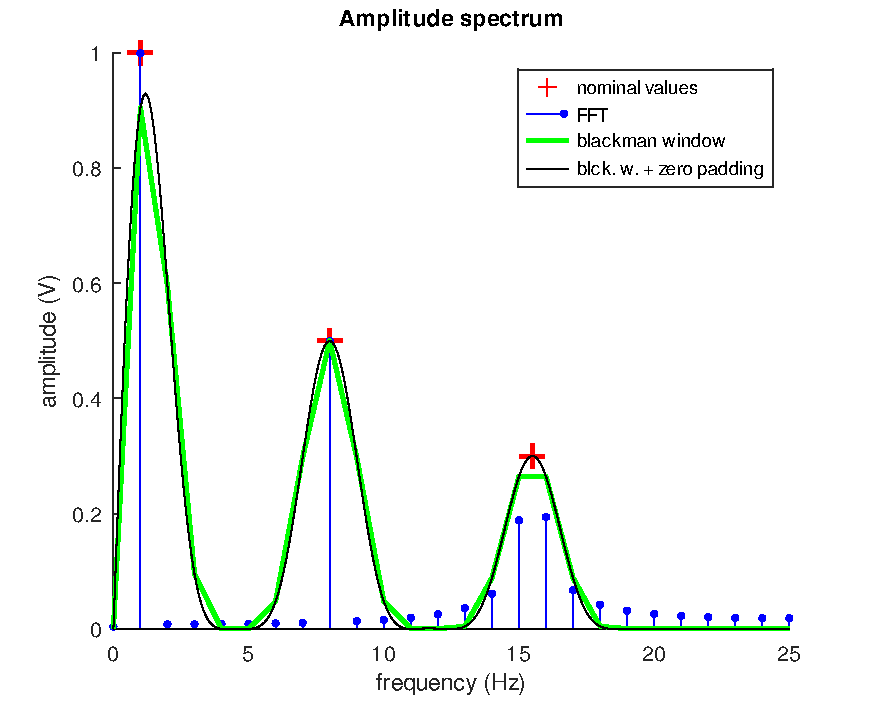
\includegraphics[width=0.7\textwidth]{algs_examples_published/SP-WFFT_alg_example-1.pdf}
\end{center}
\begin{center}
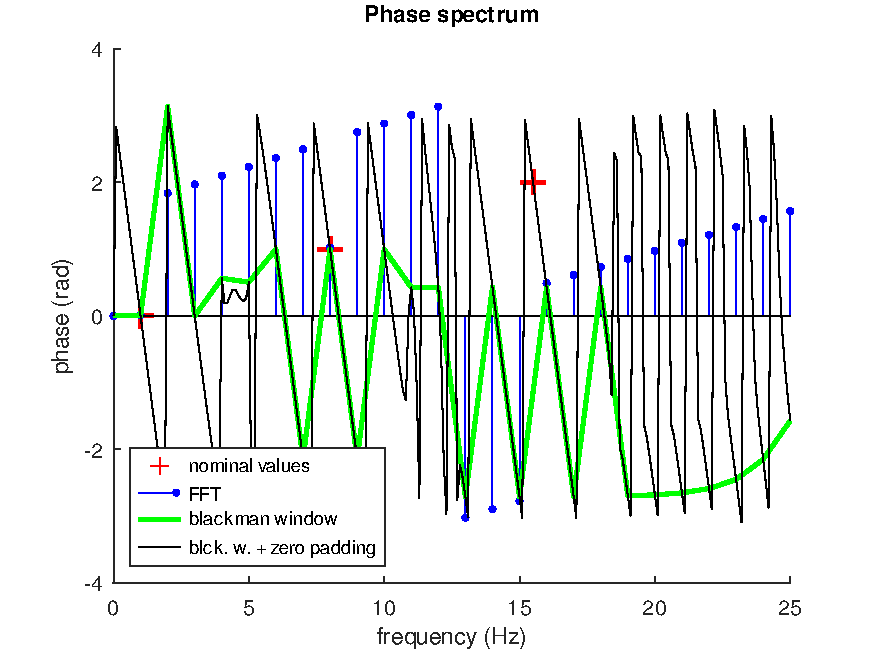
\includegraphics[width=0.7\textwidth]{algs_examples_published/SP-WFFT_alg_example-2.pdf}
\end{center}


\phantomsection
\addcontentsline{toc}{section}{Compare window coefficients}
\subsubsection*{Compare window coefficients}



Different windows has different peak widths, heights of side lobes and side lobes
roll off ratio. To see the window differences a zero padding is used.
First a simple signal of ones is prepared and zero padding is specified to 100x the length of
signal. Next for every window a spectrum is calculated and plotted.

\begin{lstlisting}
clear DI
DI.y.v = ones(1,10);
DI.fs.v = 1;
DI.fft_padding.v = 100.*length(DI.y.v);
avail_windows = {'barthann' 'bartlett' 'blackman' 'blackmanharris' 'blackmannuttall' 'bohman' 'cheb' 'flattop_matlab' 'flattop_SFT3F' 'flattop_SFT4F' 'flattop_SFT5F' 'flattop_SFT3M' 'flattop_SFT4M' 'flattop_SFT5M' 'flattop_248D' 'gaussian' 'hamming' 'hanning' 'kaiser' 'nuttall' 'parzen' 'rect' 'triang' 'tukey' 'welch'};
col = jet(length(avail_windows));
figure; hold on;
for i = 1:length(avail_windows)
        DI.window.v = avail_windows{i};
        DO = qwtb('SP-WFFT', DI);
        plot(DO.A.v, '-', 'color', col(i,:));
end
h=legend(avail_windows);
h=legend('location','eastoutside');
set(h,'FontSize',8, 'interpreter','none');
xlabel('FFT bin * 100');
ylabel('amplitude');
hold off;
\end{lstlisting}
\begin{lstlisting}[language={},xleftmargin=5pt,frame=none]
QWTB: no uncertainty calculation
QWTB: no uncertainty calculation
QWTB: no uncertainty calculation
QWTB: no uncertainty calculation
QWTB: no uncertainty calculation
QWTB: no uncertainty calculation
QWTB: no uncertainty calculation
QWTB: no uncertainty calculation
QWTB: no uncertainty calculation
QWTB: no uncertainty calculation
QWTB: no uncertainty calculation
QWTB: no uncertainty calculation
QWTB: no uncertainty calculation
QWTB: no uncertainty calculation
QWTB: no uncertainty calculation
QWTB: no uncertainty calculation
QWTB: no uncertainty calculation
QWTB: no uncertainty calculation
QWTB: no uncertainty calculation
QWTB: no uncertainty calculation
QWTB: no uncertainty calculation
QWTB: no uncertainty calculation
QWTB: no uncertainty calculation
QWTB: no uncertainty calculation
QWTB: no uncertainty calculation

\end{lstlisting}
\begin{center}
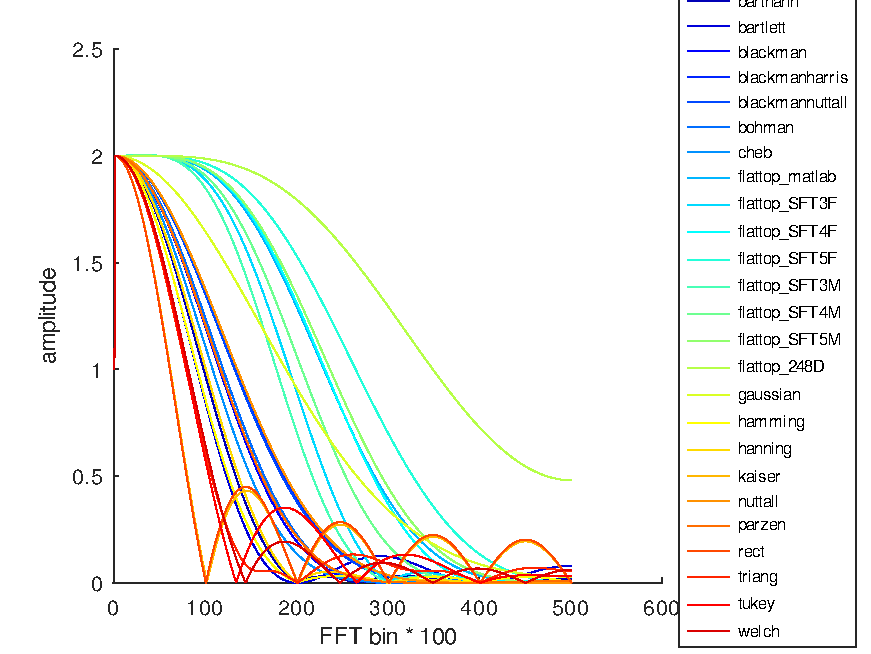
\includegraphics[width=0.7\textwidth]{algs_examples_published/SP-WFFT_alg_example-3.pdf}
\end{center}


\stopcontents[localtoc]

\resumecontents[maintoc]

\chapter{SplineResample -- Spline Resample} %<<<1 ------------------------------
\chaptermark{SplineResample}
\stopcontents[maintoc]
% included files are automatically generated by info_all_algs.m script and by Matlab publish
% function and converted by bash script betterpublish.
\section*{\infosection} %<<<2 -------------------
\begin{tightdesc}
\item [Id:] SplineResample
\item [Name:] resampling name
\item [Description:] Splines are used to resample sampled data to a new sampling frequency.
\item [Citation:] no citation
\item [Remarks:] no remark
\item [License:] no license
\item [Provides GUF:] no
\item [Provides MCM:] no
\item [Input Quantities] \rule{0em}{0em}
    \begin{tightdesc}
    \item [Required:] 
        \textsf{Ts} or \textsf{fs} or \textsf{t},\enspace \textsf{y},\enspace \textsf{fest}
    \item [Optional:] 
        \textsf{method},\enspace \textsf{D}
    \item [Parameters:] 
        \textsf{method},\enspace \textsf{D}
    \item [Descriptions:] \rule{0em}{0em}
        \begin{tightdesc}
            \item[\textsf{D}] -- Denominator to reduce resampled bandwidth
            \item[\textsf{Ts}] -- Sampling period
            \item[\textsf{fest}] -- Estimate of fundamental component frequency
            \item[\textsf{fs}] -- Sampling frequency
            \item[\textsf{method}] -- Method of resampling: `keepN`, `minimizefs`, `poweroftwo`
            \item[\textsf{t}] -- Time series
            \item[\textsf{y}] -- Sampled values
        \end{tightdesc}
    \end{tightdesc}
\item [Output Quantities:] \rule{0em}{0em}
    \begin{tightdesc}
        \item[\textsf{Pf}] -- Integer upsampling factor
        \item[\textsf{Qf}] -- Integer decimation factor
        \item[\textsf{Ts}] -- Sampling period after resampling, equal to fsest.
        \item[\textsf{fs}] -- Sampling frequency after resampling, equal to fsest.
        \item[\textsf{method}] -- Method of resampling.
        \item[\textsf{t}] -- Time series after resampling, equal to test
        \item[\textsf{y}] -- Resampled samples
    \end{tightdesc}
\end{tightdesc}

\section*{\examplesection} %<<<2 ------------------------
\startcontents[localtoc]
\printcontents[localtoc]{}{0}{\subsection*{Contents}\setcounter{tocdepth}{2}}



\phantomsection
\addcontentsline{toc}{section}{Generate sampled data}
\subsubsection*{Generate sampled data}



Three quantities have to be prepared: time series \texttt{t} and signal \texttt{y},
representing 2000 samples of sinus waveform of nominal frequency 49.77 Hz, nominal
amplitude 1 V and nominal phase 0 rad, sampled with sampling period 0.25 ms.
Signal simulates non-coherent sampling.

\begin{lstlisting}
f = 49.77;
A = 1;
N = 2000;
fs = 4000;
Ts = 1/fs;
Sampled.t.v = [0 : N-1] * Ts;
Sampled.y.v = A*sin(2 * pi * f * Sampled.t.v);
\end{lstlisting}


\phantomsection
\addcontentsline{toc}{section}{Signal frequency estimate}
\subsubsection*{Signal frequency estimate}



Get estimate of signal frequency to be coherent after resampling. For
example, algorithm PSFE can be used:

\begin{lstlisting}
Estimate = qwtb('PSFE', Sampled);
Sampled.fest.v = Estimate.f.v;
\end{lstlisting}
\begin{lstlisting}[language={},xleftmargin=5pt,frame=none]
QWTB: no uncertainty calculation
QWTB: PSFE wrapper: sampling time was calculated from time series

\end{lstlisting}


\phantomsection
\addcontentsline{toc}{section}{Call algorithm}
\subsubsection*{Call algorithm}

\begin{lstlisting}
Resampled = qwtb('SplineResample', Sampled);
\end{lstlisting}
\begin{lstlisting}[language={},xleftmargin=5pt,frame=none]
QWTB: no uncertainty calculation
QWTB: SplineResample wrapper: sampling time was calculated from time series

\end{lstlisting}


\phantomsection
\addcontentsline{toc}{section}{Get spectra}
\subsubsection*{Get spectra}

\begin{lstlisting}
SpectrumNonCoherent = qwtb('SP-WFFT', Sampled);
SpectrumResampled = qwtb('SP-WFFT', Resampled);
\end{lstlisting}
\begin{lstlisting}[language={},xleftmargin=5pt,frame=none]
QWTB: no uncertainty calculation
QWTB: SP-WFFT wrapper: sampling frequency was calculated from time series
warning: QWTB: value of quantity `y` is column vector, it was automatically transposed.
warning: called from
    qwtb>check_gen_datain at line 969 column 25
    qwtb>check_and_run_alg at line 342 column 16
    qwtb at line 114 column 47
    publish>eval_code_helper at line 1079 column 8
    publish>eval_code at line 995 column 30
    publish at line 402 column 9
    all_algs_examples2tex at line 51 column 5
 
QWTB: no uncertainty calculation

\end{lstlisting}


\phantomsection
\addcontentsline{toc}{section}{Compare estimated amplitudes}
\subsubsection*{Compare estimated amplitudes}

\begin{lstlisting}
printf('Frequency and amplitude of main signal component.\n');
printf('Simulated:                      f = %.2f, A = %.5f\n', f, A)
id = find(SpectrumNonCoherent.A.v == max(SpectrumNonCoherent.A.v));
printf('As estimated\n')
printf('Non coherent sampling and FFT:  f = %.2f, A = %.5f\n', SpectrumNonCoherent.f.v(id), SpectrumNonCoherent.A.v(id));
id = find(SpectrumResampled.A.v == max(SpectrumResampled.A.v));
printf('Resampled to coherent and FFT: f = %.2f, A = %.5f\n', SpectrumResampled.f.v(id), SpectrumResampled.A.v(id));
\end{lstlisting}
\begin{lstlisting}[language={},xleftmargin=5pt,frame=none]
Frequency and amplitude of main signal component.
Simulated:                      f = 49.77, A = 1.00000
As estimated
Non coherent sampling and FFT:  f = 50.00, A = 0.97996
Resampled to coherent and FFT: f = 49.77, A = 1.00000

\end{lstlisting}


\phantomsection
\addcontentsline{toc}{section}{Plot}
\subsubsection*{Plot}

\begin{lstlisting}
hold on
semilogy(f, A, 'xk')
semilogy(SpectrumNonCoherent.f.v, abs(SpectrumNonCoherent.A.v), '-k')
semilogy(SpectrumResampled.f.v, abs(SpectrumResampled.A.v), '-r')
hold off
xlabel('Frequency (Hz)')
ylabel('Signal amplitude')
legend('Simulated signal', 'FFT spectrum', 'Resampled and FFT spectrum')
title('Signal spectra')
\end{lstlisting}
\begin{center}
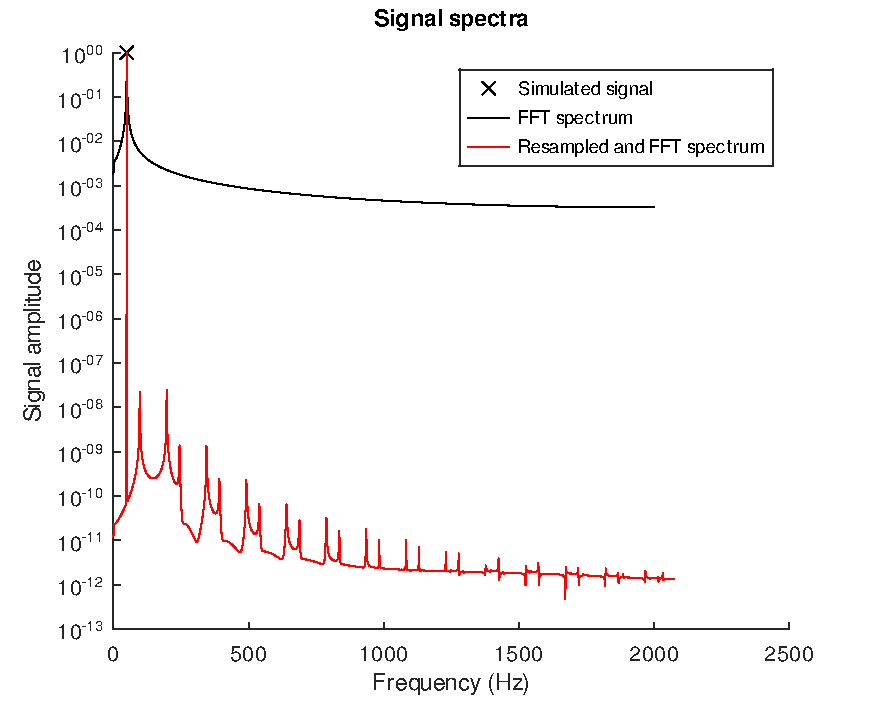
\includegraphics[width=0.7\textwidth]{algs_examples_published/SplineResample_alg_example-1.pdf}
\end{center}


\stopcontents[localtoc]

\resumecontents[maintoc]

\chapter{ThreePSF -- Standard Three Parameter Sine Wave Fit according IEEE Std 1241-2000} %<<<1 ------------------------------
\chaptermark{ThreePSF}
\stopcontents[maintoc]
% included files are automatically generated by info_all_algs.m script and by Matlab publish
% function and converted by bash script betterpublish.
\section*{\infosection} %<<<2 -------------------
\begin{tightdesc}
\item [Id:] ThreePSF
\item [Name:] Standard Three Parameter Sine Wave Fit according IEEE Std 1241-2000
\item [Description:] Fits a sine wave to the recorded data using 3 parameter (amplitude, phase and offset) model. The algorithm is according IEEE Standard for Terminology and Test methods for Analog-to-Digital Converters 1241-2000. Algorithm requires exact value of signal frequency.
\item [Citation:] IEEE Std 1241-2000, Source code from: Rado Lapuh, "Sampling with 3458A, Understanding, Programming, Sampling and Signal Processing", ISBN 978-961-94476-0-4, 1st. ed., Ljubljana, Left Right d.o.o., 2018
\item [Remarks:] If sampling time |Ts| is not supplied, wrapper will calculate |Ts| from sampling frequency |fs| or if not supplied, mean of differences of time series |t| is used to calculate |Ts|.
\item [License:] UNKNOWN
\item [Provides GUF:] no
\item [Provides MCM:] no
\item [Input Quantities] \rule{0em}{0em}
    \begin{tightdesc}
    \item [Required:] 
        \textsf{Ts} or \textsf{fs} or \textsf{t},\enspace \textsf{f}
    \item [Descriptions:] \rule{0em}{0em}
        \begin{tightdesc}
            \item[\textsf{Ts}] -- Sampling time
            \item[\textsf{f}] -- Signal frequency
            \item[\textsf{fs}] -- Sampling frequency
            \item[\textsf{t}] -- Time series
        \end{tightdesc}
    \end{tightdesc}
\item [Output Quantities:] \rule{0em}{0em}
    \begin{tightdesc}
        \item[\textsf{A}] -- Amplitude of main signal component
        \item[\textsf{O}] -- Offset of signal
        \item[\textsf{ph}] -- Phase of main signal component
    \end{tightdesc}
\end{tightdesc}

\section*{\examplesection} %<<<2 ------------------------
\startcontents[localtoc]
\printcontents[localtoc]{}{0}{\subsection*{Contents}\setcounter{tocdepth}{2}}



\phantomsection
\addcontentsline{toc}{section}{Generate sample data}
\subsubsection*{Generate sample data}



Two quantities are prepared: \texttt{t} and \texttt{y}, representing 1 second of sinus waveform of nominal
frequency 1 kHz, nominal amplitude 1 V, nominal phase 1 rad and offset 1 V sampled at sampling
frequency 10 kHz.

\begin{lstlisting}
DI = [];
Anom = 2; fnom = 100; phnom = 1; Onom = 0.2;
t = [0:1/1e4:1-1/1e4];
DI.y.v = Anom*sin(2*pi*fnom*t + phnom) + Onom;
DI.Ts.v = 1e-4;
DI.f.v = fnom;
\end{lstlisting}


\phantomsection
\addcontentsline{toc}{section}{Call algorithm}
\subsubsection*{Call algorithm}



Use QWTB to apply algorithm \texttt{ThreePSF} to data \texttt{DI}.

\begin{lstlisting}
CS.verbose = 1;
DO = qwtb('ThreePSF', DI, CS);
\end{lstlisting}
\begin{lstlisting}[language={},xleftmargin=5pt,frame=none]
QWTB: no uncertainty calculation

\end{lstlisting}


\phantomsection
\addcontentsline{toc}{section}{Display results}
\subsubsection*{Display results}



Results is the amplitude, phase and offset of sampled waveform.

\begin{lstlisting}
A = DO.A.v
ph = DO.ph.v
O = DO.O.v
\end{lstlisting}
\begin{lstlisting}[language={},xleftmargin=5pt,frame=none]
A = 2.0000
ph = 1.0000
O = 0.2000

\end{lstlisting}


Errors of estimation in parts per milion:

\begin{lstlisting}
Aerrppm = (DO.A.v - Anom)/Anom .* 1e6
pherrppm = (DO.ph.v - phnom)/phnom .* 1e6
Oerrppm = (DO.O.v - Onom)/Onom .* 1e6
\end{lstlisting}
\begin{lstlisting}[language={},xleftmargin=5pt,frame=none]
Aerrppm = 4.4409e-10
pherrppm = 2.2204e-09
Oerrppm = 1.9429e-09

\end{lstlisting}


\stopcontents[localtoc]

\resumecontents[maintoc]

\chapter{WaveformGenerator -- Waveform Generator} %<<<1 ------------------------------
\chaptermark{WaveformGenerator}
\stopcontents[maintoc]
% included files are automatically generated by info_all_algs.m script and by Matlab publish
% function and converted by bash script betterpublish.
\section*{\infosection} %<<<2 -------------------
\begin{tightdesc}
\item [Id:] WaveformGenerator
\item [Name:] 
\item [Description:] Complex waveform generator with harmonics, interharmonics, modulation abilities, reference output and reference values for phasor measurement units.
\item [Citation:] First version of the algorithm: U. Pogliano, J.-P. Braun, B. Voljc, and R. Lapuh, ‘Software Platform for PMU Algorithm Testing’, IEEE Transactions on Instrumentation and Measurement, vol. 62, no. 6, pp. 1400–1406, Jun. 2013, doi: 10.1109/TIM.2013.2239051.
\item [Remarks:] If sampling time |Ts| is not supplied, wrapper will calculate |Ts| from sampling frequency |fs| or if not supplied, mean of differences of time series |t| is used to calculate |Ts|. First frequency in |f| is considered as the main signal frequency. Modulation is not yet ready.
\item [License:] MIT License
\item [Provides GUF:] no
\item [Provides MCM:] no
\item [Input Quantities] \rule{0em}{0em}
    \begin{tightdesc}
    \item [Required:] 
        \textsf{Ts} or \textsf{fs} or \textsf{t},\enspace \textsf{L},\enspace \textsf{f},\enspace \textsf{A},\enspace \textsf{ph}
    \item [Optional:] 
        \textsf{l},\enspace \textsf{Fs}
    \item [Descriptions:] \rule{0em}{0em}
        \begin{tightdesc}
            \item[\textsf{A}] -- Amplitude of signal components
            \item[\textsf{Fs}] -- PMU frames per second
            \item[\textsf{L}] -- Number of samples
            \item[\textsf{Ts}] -- Sampling time
            \item[\textsf{f}] -- Frequency of signal components
            \item[\textsf{fs}] -- Sampling frequency
            \item[\textsf{l}] -- Number of samples before t=0
            \item[\textsf{ph}] -- Phase of signal components
            \item[\textsf{t}] -- Time series
        \end{tightdesc}
    \end{tightdesc}
\item [Output Quantities:] \rule{0em}{0em}
    \begin{tightdesc}
        \item[\textsf{t}] -- Time stamps
        \item[\textsf{y}] -- Samples
    \end{tightdesc}
\end{tightdesc}

\section*{\examplesection} %<<<2 ------------------------
\startcontents[localtoc]
\printcontents[localtoc]{}{0}{\subsection*{Contents}\setcounter{tocdepth}{2}}



\phantomsection
\addcontentsline{toc}{section}{Set acquisition properties}
\subsubsection*{Set acquisition properties}



First acquisition quantities are prepared: sampling frequency \texttt{fs} set to
10 kHz, and length of the record \texttt{L} set to 1000, representing 0.1 s long record.

\begin{lstlisting}
DI = [];
DI.fs.v = 1e4;
DI.L.v = 1e3;
\end{lstlisting}


\phantomsection
\addcontentsline{toc}{section}{Set waveform properties}
\subsubsection*{Set waveform properties}



The actual waveform will consist of 3 signal components. Main signal
component frequency will be 50 Hz, amplitude 1 V. Third harmonic amplitude
will be set to 0.15 V. Last component will be interharmonic of frequency 79 Hz and amplitude of 0.1 V.

\begin{lstlisting}
DI.f.v =  [50  150 757];
DI.A.v =  [ 1 0.15 0.05];
DI.ph.v = [ 0    0   0];
\end{lstlisting}


\phantomsection
\addcontentsline{toc}{section}{Call algorithm}
\subsubsection*{Call algorithm}



Use QWTB to apply algorithm \texttt{WaveformGenerator} to data \texttt{DI}.

\begin{lstlisting}
CS.verbose = 1;
DO = qwtb('WaveformGenerator', DI, CS);
\end{lstlisting}
\begin{lstlisting}[language={},xleftmargin=5pt,frame=none]
QWTB: no uncertainty calculation

\end{lstlisting}


\phantomsection
\addcontentsline{toc}{section}{Display results}
\subsubsection*{Display results}



Results are the time stamps and samples.

\begin{lstlisting}
plot(DO.t.v, DO.y.v, '-+')
xlabel('t (s)')
title('Waveform generated by WaveformGenerator algorithm')
\end{lstlisting}
\begin{center}
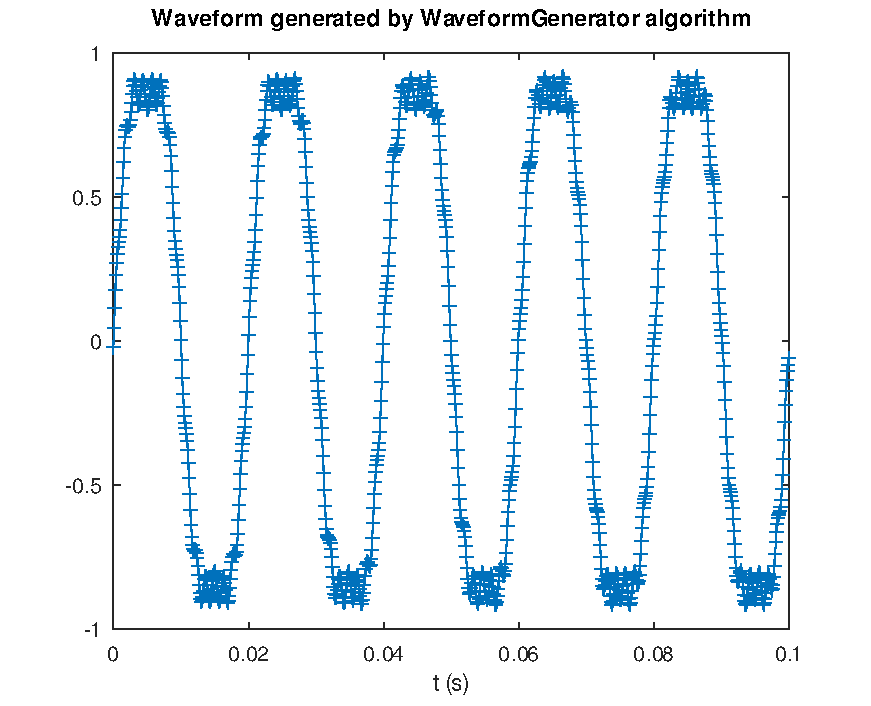
\includegraphics[width=0.7\textwidth]{algs_examples_published/WaveformGenerator_alg_example-1.pdf}
\end{center}


\stopcontents[localtoc]

\resumecontents[maintoc]

\chapter{windowedRMS -- Windowed RMS} %<<<1 ------------------------------
\chaptermark{windowedRMS}
\stopcontents[maintoc]
% included files are automatically generated by info_all_algs.m script and by Matlab publish
% function and converted by bash script betterpublish.
\section*{\infosection} %<<<2 -------------------
\begin{tightdesc}
\item [Id:] windowedRMS
\item [Name:] Windowed RMS
\item [Description:] Algorithm estimate RMS amplitude of a sampled waveform |y|. If inputs |u| (sampled voltage) and |i| (sampled current) are supplied instead of |y|, algorithms calculates not only RMS amplitudes, but also active power, apparent power, and phase between two waveforms. Possible values for |window| are: `hann`, `rect`, `bartlett`, `welch`, `hann`, `hamming`, `blackman`, `BH92`, `flattop`, `HFT70`, `HFT90D`, `HFT95`, `HFT116D`, `HFT144D`, `HFT169D`, `HFT196D`, `HFT223D`, `HFT248D`.
\item [Citation:] Rado Lapuh, "Signal Parameter Estimation using windowed RMS method"
\item [Remarks:] 
\item [License:] no license
\item [Provides GUF:] no
\item [Provides MCM:] no
\item [Input Quantities] \rule{0em}{0em}
    \begin{tightdesc}
    \item [Optional:] 
        \textsf{y},\enspace \textsf{u},\enspace \textsf{i},\enspace \textsf{window}
    \item [Parameters:] 
        \textsf{window}
    \item [Descriptions:] \rule{0em}{0em}
        \begin{tightdesc}
            \item[\textsf{i}] -- Sampled current
            \item[\textsf{u}] -- Sampled voltage
            \item[\textsf{window}] -- Name of window function
            \item[\textsf{y}] -- Sampled values
        \end{tightdesc}
    \end{tightdesc}
\item [Output Quantities:] \rule{0em}{0em}
    \begin{tightdesc}
        \item[\textsf{A}] -- RMS amplitude of a single signal
        \item[\textsf{I}] -- RMS amplitude of a current signal
        \item[\textsf{P}] -- Windowed active power
        \item[\textsf{PF}] -- Power factor
        \item[\textsf{S}] -- Windowed apparent power
        \item[\textsf{U}] -- RMS amplitude of a voltage signal
        \item[\textsf{phi\_ef}] -- Effective phase shift, acos(PF) [rad]
    \end{tightdesc}
\end{tightdesc}

\section*{\examplesection} %<<<2 ------------------------
\startcontents[localtoc]
\printcontents[localtoc]{}{0}{\subsection*{Contents}\setcounter{tocdepth}{2}}



\phantomsection
\addcontentsline{toc}{section}{Generate single sine wave sampled data}
\subsubsection*{Generate single sine wave sampled data}



The signal is not coherently sampled.

\begin{lstlisting}
DI = [];
t = (0 : 1000-1) * 1/4000;
DI.y.v = 1 * sin(2*pi * 50 * t);
\end{lstlisting}


\phantomsection
\addcontentsline{toc}{section}{Calculate RMS}
\subsubsection*{Calculate RMS}

\begin{lstlisting}
DO = qwtb('windowedRMS', DI);
\end{lstlisting}
\begin{lstlisting}[language={},xleftmargin=5pt,frame=none]
QWTB: no uncertainty calculation

\end{lstlisting}


\phantomsection
\addcontentsline{toc}{section}{Check result}
\subsubsection*{Check result}



Error of the amplitude estimate:

\begin{lstlisting}
amplitude_error = DO.A.v - 1/sqrt(2)
\end{lstlisting}
\begin{lstlisting}[language={},xleftmargin=5pt,frame=none]
amplitude_error = 3.3307e-16

\end{lstlisting}


\phantomsection
\addcontentsline{toc}{section}{Generate voltage and current sine waves}
\subsubsection*{Generate voltage and current sine waves}



If two signals are supplied representing voltage and current, power and
apparent power will be calculated.

\begin{lstlisting}
DI = [];
t = (0 : 1000-1) * 1/4000;
DI2.u.v = 1   * sin(2*pi * 50 * t + 0);
DI2.i.v = 0.5 * sin(2*pi * 50 * t + pi/4);
\end{lstlisting}


\phantomsection
\addcontentsline{toc}{section}{Calculate RMS}
\subsubsection*{Calculate RMS}

\begin{lstlisting}
DO2 = qwtb('windowedRMS', DI2);
\end{lstlisting}
\begin{lstlisting}[language={},xleftmargin=5pt,frame=none]
QWTB: no uncertainty calculation

\end{lstlisting}


\phantomsection
\addcontentsline{toc}{section}{Check result}
\subsubsection*{Check result}



Error of the voltage and current estimates:

\begin{lstlisting}
voltage_error = DO2.U.v - 1/sqrt(2)
current_error = DO2.I.v - 0.5/sqrt(2)
\end{lstlisting}
\begin{lstlisting}[language={},xleftmargin=5pt,frame=none]
voltage_error = 3.3307e-16
current_error = 4.9960e-16

\end{lstlisting}


Error of the phase estimate:

\begin{lstlisting}
phase_error = DO2.phi_ef.v - pi/4
\end{lstlisting}
\begin{lstlisting}[language={},xleftmargin=5pt,frame=none]
phase_error = 5.5511e-16

\end{lstlisting}


\stopcontents[localtoc]

\resumecontents[maintoc]

\chapter{wlsfit -- Weighted Least Square Fitting Algortihm} %<<<1 ------------------------------
\chaptermark{wlsfit}
\stopcontents[maintoc]
% included files are automatically generated by info_all_algs.m script and by Matlab publish
% function and converted by bash script betterpublish.
\section*{\infosection} %<<<2 -------------------
\begin{tightdesc}
\item [Id:] wlsfit
\item [Name:] Weighted Least Square Fitting Algortihm
\item [Description:] Least Square fitting algortihm using ordinary (OLS) or weighted (WLS) fitting on a n-positive polynomial order. If uncertainty of |y| is defined, WLS is used. If value of |w| is defined, it is used instead of unc. of |y|. If no |w| nor unc. of |y|, OLS is used.
\item [Citation:] 
\item [Remarks:] Implemented by Ricardo Iuzzolino, Estefania Luna, INTI
\item [License:] MIT License
\item [Provides GUF:] yes
\item [Provides MCM:] no
\item [Input Quantities] \rule{0em}{0em}
    \begin{tightdesc}
    \item [Required:] 
        \textsf{x},\enspace \textsf{y},\enspace \textsf{n}
    \item [Optional:] 
        \textsf{w}
    \item [Parameters:] 
        \textsf{n},\enspace \textsf{w}
    \item [Descriptions:] \rule{0em}{0em}
        \begin{tightdesc}
            \item[\textsf{n}] -- Degree of the polynomial for the regression (n>0)
            \item[\textsf{w}] -- Weigths - if defined, y.u is replaced by weights. If not defined, y.u is used as weghts.
            \item[\textsf{x}] -- Reference values
            \item[\textsf{y}] -- Observed or measured values, y.u is used as weights for the case of WLS
        \end{tightdesc}
    \end{tightdesc}
\item [Output Quantities:] \rule{0em}{0em}
    \begin{tightdesc}
        \item[\textsf{coefs}] -- Fitted coefficients
        \item[\textsf{exponents}] -- Exponents of polynomial used to fit
        \item[\textsf{func}] -- Anonymous function constructed for exponents with parameters `x` and `coefs.v`
        \item[\textsf{model}] -- Model used for calculation.
        \item[\textsf{yhat}] -- Fitted values y
    \end{tightdesc}
\end{tightdesc}

\section*{\examplesection} %<<<2 ------------------------
\startcontents[localtoc]
\printcontents[localtoc]{}{0}{\subsection*{Contents}\setcounter{tocdepth}{2}}



\phantomsection
\addcontentsline{toc}{section}{Set example data}
\subsubsection*{Set example data}



Set independent and dependent variables for \texttt{wlsfit} algorithm, OLS method.
Lets operate in semi logarithm space for easy plotting.

\begin{lstlisting}
DIols = [];
DIols.x.v = log10([10 1e2 1e3 1e4 1e5]);
DIols.x.u = [];
DIols.y.v = [19.700 32.700 69.700 90.700 148.700];
% polynomial order:
DIols.n.v = 2;

% Create data for WLS method (add uncertainties of y):
DIwls = DIols;
DIwls.y.u = [4 10 13 20 33];
\end{lstlisting}


\phantomsection
\addcontentsline{toc}{section}{Call algorithm}
\subsubsection*{Call algorithm}



Use QWTB to apply algorithm \texttt{wlsfit} to data \texttt{DIwls}.

\begin{lstlisting}
DOols = qwtb('wlsfit', DIols);
DOwls = qwtb('wlsfit', DIwls);
\end{lstlisting}
\begin{lstlisting}[language={},xleftmargin=5pt,frame=none]
QWTB: no uncertainty calculation
QWTB: wlsfit wrapper: No y uncertainties nor weights -> using OLS fitting
QWTB: no uncertainty calculation
QWTB: wlsfit wrapper: Using WLS fitting based on y uncertainties.

\end{lstlisting}


\phantomsection
\addcontentsline{toc}{section}{Display results}
\subsubsection*{Display results}



Results is

\begin{lstlisting}
disp('')
disp([DOols.model.v ':'])
disp(['offset          : ' num2str(DOols.coefs.v(1)) ' +- ' num2str(DOols.coefs.u(1))])
disp(['linear coeff.   : ' num2str(DOols.coefs.v(2)) ' +- ' num2str(DOols.coefs.u(2))])
disp(['quadratic coeff.: ' num2str(DOols.coefs.v(3)) ' +- ' num2str(DOols.coefs.u(3))])
disp([DOwls.model.v ':'])
disp(['offset          : ' num2str(DOwls.coefs.v(1)) ' +- ' num2str(DOwls.coefs.u(1))])
disp(['linear coeff.   : ' num2str(DOwls.coefs.v(2)) ' +- ' num2str(DOwls.coefs.u(2))])
disp(['quadratic coeff.: ' num2str(DOwls.coefs.v(3)) ' +- ' num2str(DOwls.coefs.u(3))])
\end{lstlisting}
\begin{lstlisting}[language={},xleftmargin=5pt,frame=none]

Ordinary Least Squares:
offset          : 14.5 +- 2.1448
linear coeff.   : -0.11429 +- 1.6345
quadratic coeff.: 5.2857 +- 0.26726
Weighted Least Squares, weights based on u(y):
offset          : 12.6828 +- 16.9884
linear coeff.   : 1.9434 +- 19.1198
quadratic coeff.: 4.9055 +- 3.9754

\end{lstlisting}


\phantomsection
\addcontentsline{toc}{section}{Interpolate values}
\subsubsection*{Interpolate values}



Interpolate fitted polynom at values \texttt{t}.

\begin{lstlisting}
t = [0:0.1:6];
tyols = DOols.func.v(t, DOols.coefs.v);
tywls = DOwls.func.v(t, DOwls.coefs.v);
\end{lstlisting}


Calculate uncertainties of interpolated values (\texttt{S} is sensitivity matrix, \texttt{CC} is covariance
matrix of coefficients, \texttt{CT} is covariance matrix of interpolated values, \texttt{uty} is uncertainty of
interpolated values).

\begin{lstlisting}
for i = 1:length(t);
        S = t(i).^[0:DIols.n.v];
        CC = diag(DOols.coefs.u,0)*DOols.coefs.c*diag(DOols.coefs.u,0);
        CT(i)=S*CC*S';
end
utyols=CT.^0.5;

for i = 1:length(t);
        S = t(i).^[0:DIwls.n.v];
        CC = diag(DOwls.coefs.u,0)*DOwls.coefs.c*diag(DOwls.coefs.u,0);
        CT(i)=S*CC*S';
end
utywls=CT.^0.5;
\end{lstlisting}


\phantomsection
\addcontentsline{toc}{section}{Plot results}
\subsubsection*{Plot results}

\begin{lstlisting}
hold on
% input data:
errorbar(DIwls.x.v, DIwls.y.v, DIwls.y.u, 'xb')
% outputs:
plot(DIols.x.v, DOols.yhat.v, 'or')
errorbar(DIwls.x.v, DOwls.yhat.v, DOwls.yhat.u, 'og')
plot(t, tyols, '--r');
plot(t, tywls, '-g');
plot(t, tyols + utyols, '--r');
plot(t, tywls + utywls, '-g');
plot(t, tyols - utyols, '--r');
plot(t, tywls - utywls, '-g');
xlabel('log(f)')
ylabel('error of amplitude')
legend('original data','fitted values, OLS', 'fitted values, WLS','interpolated values, OLS', 'interpolated values, WLS', 'uncer. of int. val., OLS', 'uncert. of int. val., WLS','location','southeast')
hold off
\end{lstlisting}
\begin{center}
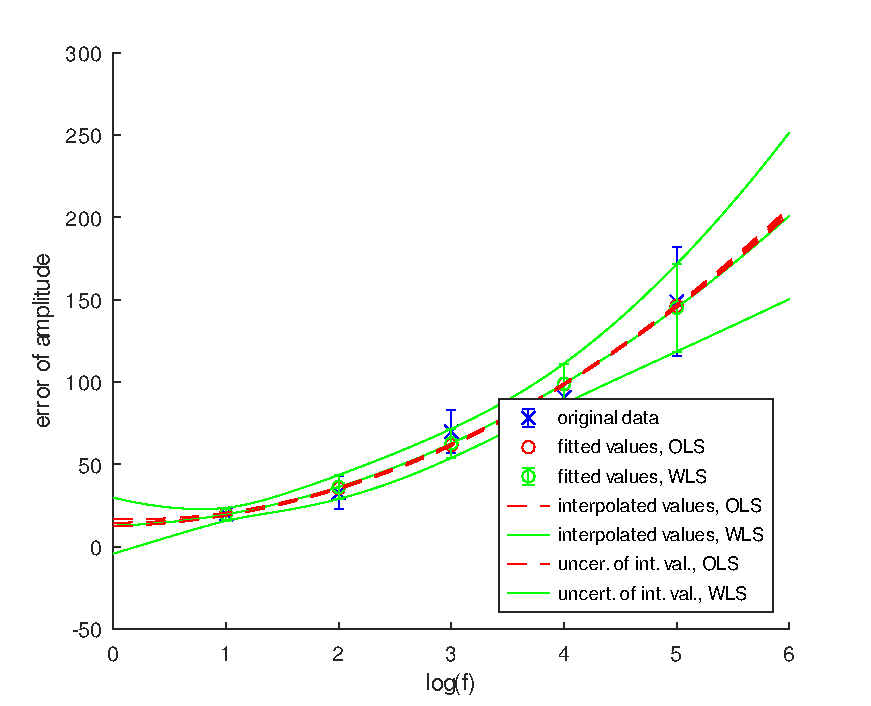
\includegraphics[width=0.7\textwidth]{algs_examples_published/wlsfit_alg_example-1.pdf}
\end{center}


\stopcontents[localtoc]

\resumecontents[maintoc]

\end{document}

% vim settings: vim:foldmarker=%<<<,%>>> fdm=marker fen
